\documentclass[12pt]{ujreport}
\usepackage{comment}
\usepackage{./sty/eclepsf}
\usepackage{tascmac}
\usepackage{tabularx}
\usepackage{listliketab}
\usepackage[longnamesfirst]{natbib}
\usepackage[dvipdfmx]{graphics}
\usepackage[dvipdfmx]{graphicx}
\usepackage[dvipdfmx]{color}
\usepackage{subfigure}
\usepackage{alltt}
\usepackage{here}
\usepackage{afterpage}
\usepackage{./sty/ncodeline}
\usepackage{url}  

%\usepackage[dvipdfmx, colorlinks, breaklinks,%
\usepackage[dvipdfmx, breaklinks,%
bookmarks=true, bookmarksnumbered=true,%
bookmarkstype=toc, bookmarksopen=true,bookmarksopenlevel=3,%
pdftitle={RG},%
]{hyperref}
\usepackage{bookmark}

\AtBeginDvi{\special{pdf:tounicode EUC-UCS2}}

\usepackage{fancyhdr}

\usepackage{./sty/doxygenorig}

\usepackage{indentfirst}
\usepackage{listings,./sty/jlisting}
\usepackage{algorithm}
\usepackage{algpseudocode}
\usepackage{multicol}
\def\lstlistingname{ソースコード}

\lstset{%
 language={C++},
 %backgroundcolor={\color[gray]{.85}},%
 basicstyle={\small\ttfamily},%
 identifierstyle={\small},%
 commentstyle={\small\itshape},%
 keywordstyle={\small\bfseries},%
 ndkeywordstyle={\small\ttfamily},%
 stringstyle={\small\ttfamily},
 frame={tb},
 framesep=1zw,
 breaklines=true,
 numbers=left,%
 xrightmargin=0zw,%
 xleftmargin=1.5zw,%
 numberstyle={\scriptsize},%
 stepnumber=1,
 numbersep=1zw,%
 lineskip=-0.5ex%
}

\usepackage{amssymb}
%\usepackage{supertabular,multirow}

\usepackage{array}
\newcolumntype{M}[1]{>{\centering\arraybackslash}m{#1}}

% A4  size: 297mm*210mm %1pt = 0.35mm
\setlength{\topmargin}{-3.4mm} % 10pt 25.4mm - 3.4mm = 22mm
\setlength{\oddsidemargin}{-0.4mm} % 25.4mm - 0.4mm = 25mm
\setlength{\evensidemargin}{-0.4mm} % 25.4mm - 0.4mm = 25mm
\setlength{\textheight}{231mm} % 660pt % original is 225.75mm 645pt
\setlength{\textwidth}{160mm} % 457pt

\renewcommand{\topfraction}{.99}
\renewcommand{\textfraction}{.0}
\renewcommand{\floatpagefraction}{.99}
\renewcommand{\bibname}{参考文献}

\usepackage{tikz}
\newcommand*\circled[1]{\tikz[baseline=(char.base)]{
            \node[shape=circle,draw,inner sep=1pt] (char) {#1};}}
\pagestyle{fancy}
\lhead[]{}

\makeatletter
\def\chaptermark#1{\markboth {\ifnum \c@secnumdepth>\m@ne
\@chapapp\ \thechapter \@chappos\ \fi #1}{}}
\makeatother

% タイトル
\def\title{トポロジー変化に耐性のある宇宙インターネットのコンタクト情報配布手法の実装と評価(仮)}
% 英語タイトル
\def\etitle{Implementation and Evaluation of Contact Information Distribution Methods in the Space Internet (tentative)}
% 著者(日本語)
\def\author{鈴木 翔太}
% 著者(英語)
\def\eauthor{Shota Suzuki}
% 学部・研究科
\def\dept{慶應義塾大学 環境情報学部}
% 学部・研究科(英語)
\def\edept{Keio University Bachelor of Arts in Environment and Information Studies}

\usepackage{hyperref} 
\begin{document}

\pagenumbering{roman}
\begin{titlepage}
  \begin{center}
    \begin{large}
      卒業論文   2023年度(令和5年度)\\
      \vspace{24pt}
      {\Huge \title}
    \end{large}
  \end{center}
  \vspace{40em}
  \begin{flushright}
    \large \dept\\
    \author
  \end{flushright}
\end{titlepage}

\thispagestyle{empty}


卒業論文要旨 - 2025年度(令和7年度)
\begin{center}
\begin{large}
\begin{tabular}{|M{0.97\linewidth}|}
    \hline
      \title \\
    \hline
\end{tabular}
\end{large}
\end{center}
\begin{spacing}{1.2}
\small
モバイル通信の標準化において、3GPPは仕様書ベースのプロセスを採用しているため、実装・検証が後回しになり、「仕様上は規定されているが実際には動作しない機能」が多数生じている。次世代(6G)に向けては、実装ベースの標準化(implementation-driven standardization)による早期の相互運用性検証と標準化へのフィードバックサイクルの確立が不可欠である。しかし、実機RANを用いた検証は電波法上の制約から困難であり、標準化プロセスの検証基盤が不足している。

本研究は、免許不要帯で運用可能なsXGP(TD-LTE互換)をeNBとして活用し、4GのRAN(UE・eNB)と5G Core(5GC)を接続するコンバータを実装することで、実装ベース標準化を支援する実機検証環境を提案する。本研究では、(1) sXGPを用いた法令遵守型RANの構築、(2) S1AP/NGAP/NASの信令処理とGTP-U中継を行うコンバータの設計・実装、(3) 相互運用性検証とフィードバックのための計測・再現手順の整備、を行った。

評価として、登録・PDUセッション確立などの基本機能を確認し、実機特有の相互運用性問題の検出能力を検証した。提案環境は、(a) 標準仕様の実装検証と相互運用性テスト、(b) 標準化へのタイムリーなフィードバック、(c) 継続的インテグレーション・回帰テスト、(d) 性能評価とボトルネック分析、(e) 教育・トレーニング用途、(f) プロトコル拡張の試作・検証、といったユースケースに適用可能である。本環境により、実装を動かしながら標準化を進めるサイクルを確立し、6G時代のアジャイルな標準化プロセスに貢献する。

\end{spacing}

キーワード:\\
\underline{1. モバイルシステム}
\underline{2. sXGP}
\underline{3. 5G Core}
\underline{4. Open5GS}
\underline{5. GTP-U}
\begin{flushright}
\dept \\
\author
\end{flushright}

\thispagestyle{plain}
\clearpage

Abstract of Bachelor's Thesis - Academic Year 2024
\begin{center}
\begin{large}
\begin{tabular}{|p{0.97\linewidth}|}
    \hline
      \etitle \\
    \hline
\end{tabular}
\end{large}
\end{center}

~ \\

~ \\
Keywords : \\
\underline{1. Delay/Disruption Tolerant Network} 
\underline{2. Contact Graph Routing} 
\begin{flushright}
\edept \\
\eauthor
\end{flushright}
\thispagestyle{plain}
\clearpage

\tableofcontents\thispagestyle{plain} %目次
\clearpage
\listoffigures\thispagestyle{plain} %図目次
\clearpage
\listoftables\thispagestyle{plain} %表目次
\clearpage

\pagenumbering{arabic}
\chapter{序論}
% --- 章アウトライン・TODO・参考文献引用例 ---
% この章では、研究の背景・課題・目的・本論文の貢献・構成を述べる。
% TODO: 具体的な背景事例や課題を Open5GS/sXGP-5G 実装と関連付けて記述。
% TODO: 参考文献を本文中で引用する(例: \cite{rfc5326})。
% 例: 5Gの研究環境構築に関する課題は \cite{McBrayer2022} などで議論されている。
% ------------------------------------------

\section{背景}
モバイル通信の標準化において、3GPPは仕様書を先に策定し、実装・相互運用性検証は後工程となる「仕様先行型」のプロセスを採用している。これは大規模な通信インフラの標準化として必要な側面もあるが、実装が追いつかず、「仕様上は存在するが実際には動作しない機能」や「異なる実装間での相互運用性問題」が多数生じている。一方、IETFなどインターネット技術の標準化では"rough consensus and running code"の原則に基づき、実装を動かしながら標準化を進める「実装ベース標準化」が実践されており、標準と実装の乖離が少ない。

6G時代に向けては、標準化サイクルの高速化と実装・検証の早期化が不可欠である。しかし、モバイル通信では実機RANを用いた検証が電波法上の制約から困難であり、実装ベース標準化を支援する検証基盤が不足している。本研究は、免許不要帯で運用可能なsXGP(TD-LTE互換)をeNBとして活用し、4G RAN(UE・eNB)と5G Core(5GC)を接続するコンバータを提案することで、法令遵守の範囲で実機検証を可能にする。5GCの基本的なアーキテクチャと手順は3GPP TS~\cite{threegpp-23501,threegpp-23502}に規定されており、OSS実装としてはOpen5GS~\cite{open5gs}が広く用いられている。

\section{問題意識と課題}
本研究の背景には、以下の三点に関する強い問題意識がある。

\begin{itemize}
	\item \textbf{実装ベース標準化の不在}: 3GPPの標準化プロセスは仕様書ベースであり、実装・相互運用性検証が後回しになる。結果として「仕様上は存在するが実際には動作しない機能」「実装間での非互換性」が多数生じ、標準化へのフィードバックループが極めて遅い。IETFの"running code"原則とは対照的に、実装を動かしながら標準化を進める文化が欠如している。6G時代のアジャイルな開発・標準化サイクルを確立するには、実装ベースの検証基盤が不可欠である。

	\item \textbf{実装検証環境の不足}: モバイルコアはソフトウェア化が進み、Open Source Software(OSS)も充実してきた。しかし、実機RANを用いた検証環境は電波法上の制約から構築困難であり、OSSの相互運用性や実機特有の問題を検証する手段が限られている。シミュレータでは発見できない実装レベルの問題(タイミング、リソース競合、NIC/ドライバ依存の挙動など)を早期に検出できないことが、標準化と実装のギャップを拡大させている。

	\item \textbf{標準化フィードバックサイクルの遅延}: 現状では、仕様策定 → 実装 → 商用展開 → 問題発覚 → 次期仕様での修正、というサイクルに数年を要する。この遅延により、不具合のある仕様が長期間放置され、互換性問題が蓄積する。実機検証環境を用いた早期の相互運用性テストと標準化団体へのタイムリーなフィードバックが可能になれば、このサイクルを大幅に短縮できる。免許不要帯で運用可能なsXGPは、この課題に対する実践的な解決策となる。
\end{itemize}

これらに加えて、相互接続性、運用・再現性、計測基盤の不足といったモバイルシステム全体の横断的課題を踏まえ、とりわけRANとコア間のインターワーキングが標準化・実装検証のボトルネックである点を指摘する。

\section{研究目的}
\begin{itemize}
	\item 実装ベース標準化を支援する実機検証環境の構築方法を示す。
	\item sXGPベースの4G RANと5GCを接続するコンバータの設計・実装を通じて、標準仕様の相互運用性検証を実現する。
	\item 実機特有の問題を早期検出し、標準化へのフィードバックサイクルを短縮する手法を提案する。
	\item 再現可能な検証環境により、継続的インテグレーション・回帰テストを可能にする。
\end{itemize}

\section{本論文の貢献}
\begin{itemize}
	\item 実装ベース標準化を可能にする実機検証環境(sXGP + 5GC)の実証。標準仕様と実装の乖離を早期発見し、標準化団体へタイムリーにフィードバックする基盤を提供。
	\item 4G RANと5GCの信令・ユーザ面の相互接続に関する設計指針と、実装レベルでの相互運用性問題の分類・解決手法の整理。
	\item 再現性の高い検証プロファイル(トポロジ、計測項目、実験手順)の提示により、継続的な相互運用性テストと回帰テストを支援。
	\item 免許不要帯を活用した法令遵守型の実機検証手法の確立。電波法制約下でも実装を動かしながら標準化を進めるアプローチの実現可能性を示す。
\end{itemize}

\section{論文構成}
本論文は以下の構成である。第\ref{chap:background}章で基礎知識と課題整理、第\ref{chap:related}章で関連研究と事例、第\ref{chap:proposal}章で提案手法、第\ref{chap:experiment}章で実験環境と方法、第\ref{chap:evaluation}章で評価、第\ref{chap:conclusion}章で結論と今後の課題を述べる。


\chapter{hoge}
\section{宇宙通信におけるインターネット技術の適用性とDTN}
近年、月や火星の宇宙探査ミッションが本格化し、NASA中心のアルテミス計画citenasa2020は2025年から
有人ミッションも予定している。 これらの計画に伴い、 今後は月・火星にある衛星やさまざまな通信機器、 
デバイスなどの数が増加する可能性が高い。 従来までの宇宙ミッションにおいて宇宙のノードと地球との通信は、 
地球上にある各国の大型アンテナを利用し、 一対一の通信を行っていた。 しかしこのような計画でノードの数が増加する場合、
通信ニーズに対応するためには宇宙にも多対多のノードで通信が可能なインターネットが必要となる。 
既存のインターネットはEnd-to-Endの疎通性が確保できている環境で通信を行うことが多いが、 
宇宙で通信を行う際には頻繁な断絶と大きな遅延が問題となる。 中継ノードとなる様々な宇宙機は
宇宙空間での位置が常に変化しており、天体の影に入るなどで断絶が頻繁に起こる。また通信の際には地球月間でも片道1。3秒、 
地球火星間では太陽に対する2天体の公転の状況によって、 片道4分から20分程度の遅延が想定されている。 
End-to-EndでTCPを用いた通信を行う際には、 3-way-handshakeなどを含め
これらの天体間を複数回往復する通信を行う必要があり、遅延はさらに大きな時間になる。 

そのため宇宙のインターネットにはDelay and Disruption Tolerant Networking(DTN)の
技術を利用することが考えられている。 DTNの技術の一つにBundle Protocol(BP)があり、 
BPでは通信されるデータはバンドルという可変長のデータとして転送される。 
中間ノードでは経路上の次のノードへ転送可能なタイミングまでバンドルを蓄積することが可能になっているため、 
End-to-Endの通信疎通性が確保できていない場合でも、 この蓄積による転送を行うことにより断絶に強い通信ができる。
 またトランスポートレイヤにUDPなどのプロトコルを用いることで、 
 比較的遅延を抑えて通信することもできる。 

\subsection{Bundle Protocol}
Bundle Protocol (BP)は、DTNにおける主要な通信技術で遅延・断絶が起きやすい環境でデータを確実に伝送するために設計された。

Bundle Protocolは、 データを「バンドル」と呼ばれる可変長の単位として送信する。このバンドルは、 
送信元から目的地までの途中で複数の中継を経ても、全体としてデータを確実に届けるためのものである。 
また、このプロトコルは「ストア&フォワード」方式を利用しており、 各中継ノードが受け取ったバンドルを一時的に保存し、 
次のノードと通信できるタイミングが来るまで待機する。 これにより、通信が一時的に途絶えてもデータが失われることなく、 次のノードへと送信される。

\subsection{Convergence LayerとLTP}
DTNでは多様なプロトコルがトランスポートレイヤ以下の層で使用することを想定しており、 図 ref中のConvergence Layerは
それらの違いを吸収することを目的としている。 Convergence Layer Protocol(CLP)としては、 
利用する下位レイヤプロトコルにより、
- sTCP-based CLP (TCPCL)
- User Datagram Protocol (UDP)
- based CLP (UDPCL)、 Saratoga CLP
- Licklider Transmission Protocol (LTP)
- based CLP (LTPCL)
- Licklider Transmission Protocol(LTP)などがある。 
LTP citerfc5326はコンバージェンスレイヤのプロトコルの一つであり、 再送制御の機能も実装している。
 LTPをコンバージェンスレイヤに用いる場合、 トランスポートレイヤにUDPを用いることがあるほか、 
 宇宙での通信においてLTPが直接リンク層にアクセスすることも想定されている。
\subsection{既存のDTN実装}
既にいくつかの研究機関などによりDTN技術を実装したソフトウェアがリリースされている。 いくつかの例を以下に示す。 

% Interplanetary Overlay Network DTN(ION-DTN):NASA/JPL
% HDTN:NASA/Glenn research center
% DTN ME:Marshall Space Flight center
% μD3TN:D3TN GmbH
% IONe:Experimental ION Scott Burleigh United States 
% DTN7/Go:University of Marburg German

これらのDTNソフトウェアは、 基本的に通信内容からバンドルへのエンコード・デコード、 
中間ノードでのバンドルのままでの蓄積転送を可能にしているが、 
Convergence Layerが対応しているトランスポートレイヤプロトコルの種類などの点で異なる。 


\section{宇宙インターネットにおけるルーティング}
\subsection{衛星間のContact}
DTNは、 通信の遅延や途絶が発生する環境でデータを確実に届けるための技術である。このDTNにおいて、
 通信が可能な時間やタイミングを「Contact」と呼んでいる。 Contactとは、 
 2つのノード間で直接通信が可能な期間やその条件を指し、 データを送受信できる時間を意味している。

DTNを使用する環境では、 常に接続が確立されている訳ではなく、 ノード間の通信が可能な期間が限られていることが一般的である。
したがって、 このContactを正確に把握することが、 効率的なデータ転送やネットワークの最適化において極めて重要な要素となっている。
例えば、 地球と宇宙探査機の間の通信を考えてみると。 両者が視界に入る時間にだけデータを送信することができる。 この時間がContactにあたる。 

\subsection{Contact Graph Routing}
既に述べた通り既存のDTN実装は複数あるが、これらのDTN実装におけるルーティング手法は、
主にContact Graph Routing(CGR)が用いられ、 
CCSDSではSCHEDULE-AWARE BUNDLE ROUTINGとして標準化されている。 
宇宙におけるノード間の通信可能な機会は物理的な軌道の計算により予測可能であり、 
CGRはノードの通信可能機会とそのスループットなどが書かれたContact Planを用いて
\subsection{IPN address}
IPNアドレス(Interplanetary Networking Address)は、 DTN環境で使用されるアドレス形式で、
宇宙通信のためのネットワーク識別とエンドポイントの識別を可能にするものである。 従来のインターネットプロトコルアドレス(IPアドレス)は、
リアルタイムでの通信や短い遅延を前提とした設計であるため、 宇宙空間における遅延や断絶が発生する環境では適切に機能しない。
DTNのアーキテクチャは、 これらの遅延や断絶を前提としており、 IPネットワークとは異なる方法でデータを伝送するため、
IPNアドレスが必要とされている。 さらに、 IPNアドレスは地上のインターネットや宇宙のネットワークなど、
異なるアドレッシングスキームを持つネットワークの統合する役割としても機能する。

IPNアドレスは「ipn:ノード番号. サービス番号」という形式で記述され、 これにより特定の宇宙船や装置が個別に識別される。 

\section{宇宙でのトポロジーの変化}
\chapter{宇宙におけるコンタクト情報に関連した研究と標準化動向}

\label{chap:related_works}
\section{宇宙インターネットにおけるルーティングのアルゴリズム}
\subsection{CGRのアルゴリズム}
先行研究1: Routing in the Space Internet: A contact graph routing tutorial
CGRについて定義した論文
DTNでのrouting schemeの管理方法については、Centralized,Distributed,Source routingがあるとした上で、「in-depth quantitative comparison of the centralized, source routing and distributed routing approach remains a topic for future research.」として、配送方法についての検討の必要性が提唱されている
\subsection{Yen routing algorithm}

\section{宇宙ネットワークのシミュレーション}
宇宙ネットワークの立ち位置
既存研究・関連研究

先行研究2: Tracking Lunar Ring Road Communication
先行研究1で述べられた、DTNにおけるrouting schemeのうち、Source routingによって配送を行う、月のcubesat コンステレーションを想定。
経路を多く把握するノードを決めておき、各ノードは最低限の経路情報のみを把握
評価には配送成功率と平均配送時間のみを使用し、
上記で述べた「宇宙環境下で最も適した」かどうかについては定性的に判断しているのみ
提案(Approach)
先行研究では、Centralized,Distributedの手法についての定量的な比較が存在しない。
Centralized,Distributedの手法のどちらがより想定する宇宙環境におけるコンタクト情報配布方法として適切か、またそのための適切な条件を探索する

\section{宇宙インターネットにおける経路情報管理手法の確立の必要性}
\section{コンタクト情報から経路計算への処理を行うノード}
\subsection{Distributed Method}
コンタクトグラフそのもの
CCSDSの見本(単純な表形式)に沿って作成。

\subsection{Centralized Method}
コンタクトグラフから計算された経路情報

\chapter{Contact Planの臨時更新の惑星内への限定的な伝播の提案}
\label{chap:suggestion}
本章では、前章でContact Planの臨時更新時に述べた課題に対して、
その解決策が満たすべき要件について整理し、
Contact Planの臨時更新の際の情報拡散を惑星内に限定することを提案する。
Contact Planの臨時更新の目的は、DTNの各ノードがその時点における
ネットワークのより正確なトポロジー情報を得て、最適な経路を選択できるようにすることである。
DTNのどこかでリンク障害が起きた場合、Contact Planを



\section{Contact Planの臨時更新における要件}
ここでは、Contact Planの臨時更新において満たされるべき要件を整理する。
\subsection{要件1: 臨時更新による経路収束までに要する時間の短縮}
\subsection{要件2: リンク障害による配送遅延増加に対する臨時更新の効果}
ここでは、Contact Planの臨時更新において満たされるべき要件として、
そもそもの目的である実態とかけ離れた状態でCGRを続けることを回避し遅延を抑制すると言う目標にたいして、
情報伝搬範囲を限定することで本提案がそのメリットを損なわないかが重要であるということを述べる。




% \begin{figure}[tbh]
%     \centering
%     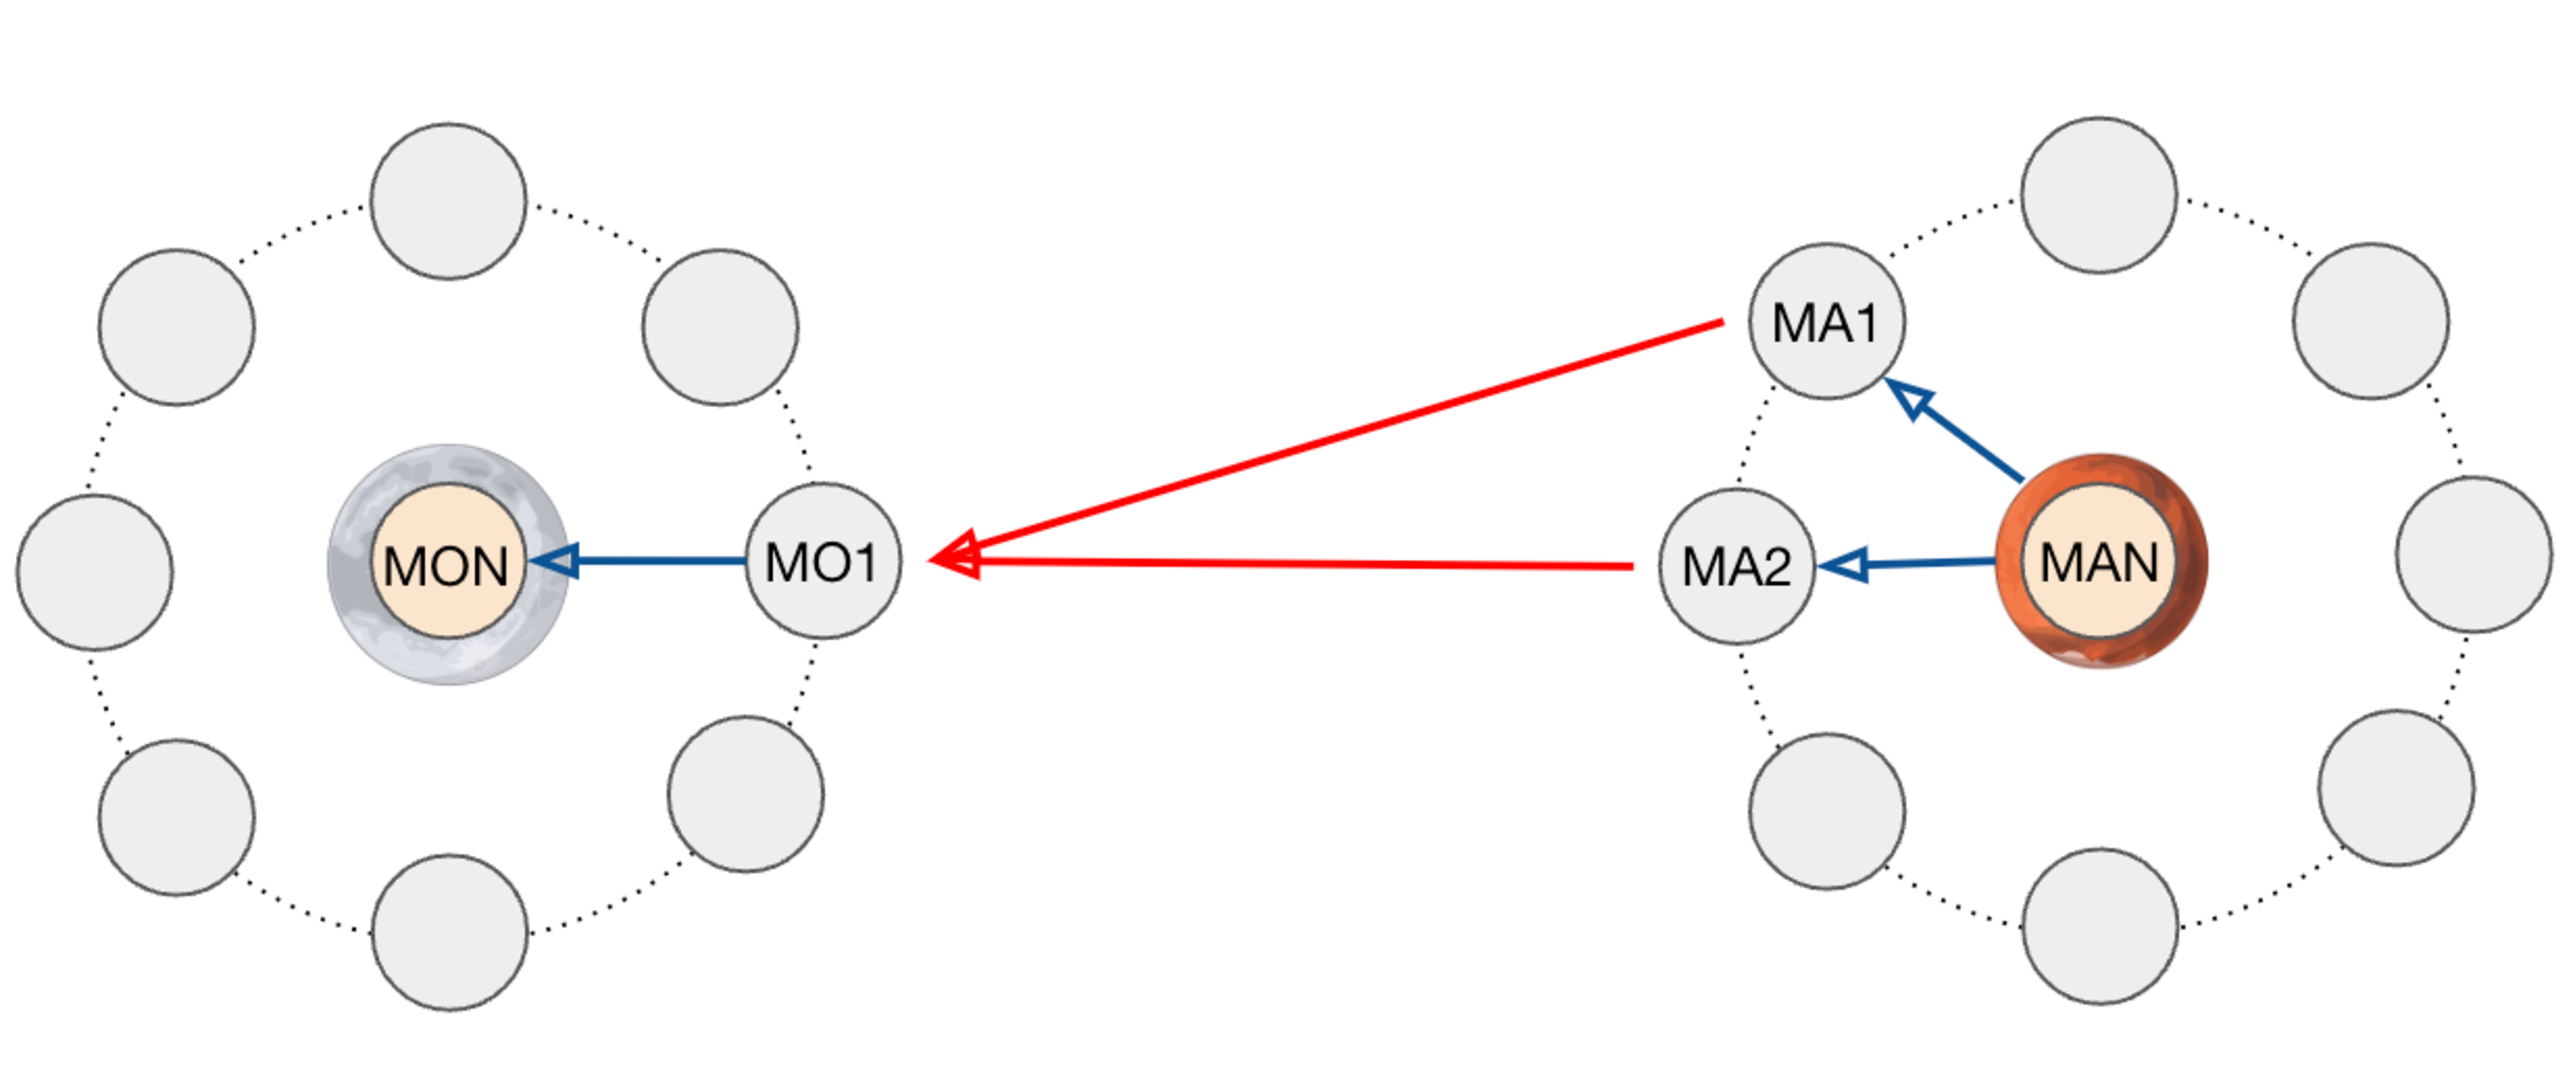
\includegraphics[width=0.7\textheight]{img/ipn_topology.pdf}
%     \caption{2040年代以降のIPNのトポロジー}
%     \label{fig:dtnprotocolstack}
%     \begin{minipage}{\textwidth}
%         \raggedright
%        2040年代以降、IPNは火星にも拡大し、地球・月・火星の3天体間でのIPNが形成される可能性が想定できる。
%     \end{minipage}
% \end{figure}

\section{要件に対する先行手法と本研究の提案手法との比較}
先行研究と本研究の提案手法の比較を行う。

\chapter{評価}
\label{chap:evaluation}
\section{評価方針}
\section{Omnet++とDTNsimを持ちいた評価環境}
\subsection{宇宙を想定した衛星ネットワークのシナリオとパラメータ}
\subsection{シミュレーションで用いるバンドルトラフィック}
\section{実験結果}
\subsection{トポロジー変化に応じたバンドルの到達率}
\subsection{Centralized,Distributedの各手法において配布されるコンタクト情報量}

\section{本章のまとめ}
\chapter{結論と展望}
\label{chap:conclusion}
\section{本研究のまとめ}
\section{今後の課題と展望}
\subsection{実際の宇宙環境により即したシミュレーション}
\subsection{DTNと深宇宙IP Networkでのルーティングの際の比較}
\chapter*{謝辞}\markboth{謝辞}{謝辞}
\addcontentsline{toc}{chapter}{謝辞}
\label{thanks}
本論文を執筆するにあたり,ご指導賜りました慶應義塾大学教授 村井純博士,慶應義塾大学環境情報学部教授 中村修博士,同学部教授 楠本博之博士,同学部教授 高汐一紀博士,同学部教授 Rodney D.Van Meter 博士,同学部教授 植原啓介博士,同学部教授 三次仁博士,
同学部教授 中澤仁博士,同学部教授 手塚悟博士,同学部教授 武田圭史博士,同学部准教授 大越匡博士,同大学政策・メディア研究科特任教授 鈴木茂哉博士,同研究科特任助教 工藤紀篤博士, 同研究科特任講師 松谷健史博士に感謝いたします.

特に植原啓介博士には rgroot のファカルティとして,日頃から研究面や運用面で指導をしていただきました.
また,1 月に参加した私にとって初めての国際会議に同伴していただき,緊張している私をサポートしていただきました.感謝いたします.

私がコンピュータネットワークの分野に進むきっかけを作っていただいた,慶應義塾大学大学院 豊田安信氏,元慶應義塾大学大学院 (現 NTT コミュニケーションズ) 深川祐太氏に感謝いたします.
私は 2020 年秋学期に開講された,インターネットの設計と運用 という講義でネットワーク技術の面白さを知ることができました.
豊田安信氏,深川祐太氏は TA/SA として私にネットワーク技術の面白さを伝えてくださりました.
また,私を rgroot に誘ってくださったのもこのお二人でした.
ありがとうございます.

東京大学准教授 中村遼博士に感謝いたします.
中村遼博士には,研究面で多大な指導をしていただきました.
研究ネタを一緒に考えてくださり,本論文のアイデアも中村遼博士からいただきました.
また,中村遼博士に指導をしていただきながら執筆した論文は ICOIN 国際会議に採択していただくことができました.感謝いたします.

慶應義塾大学修士課程 石原匠氏に感謝いたします.
石原匠氏は友人として私に接してくれながら,ときには先輩としてその背中を見せてくださりました.
コロナ禍に入学した私には大学に友人が少なかったので,先輩でありながら気軽に話せる存在は大変心の支えになりました.

東京大学大学院 伊藤広記氏,元東京大学大学院 (現 LINE ヤフー株式会社) 金谷光一郎氏に感謝いたします.
伊藤広記氏,金谷光一郎氏は,当時の私と同様にネットワーク運用未経験者として WIDE Project の vSIX ワーキンググループに参加し,共に切磋琢磨しあって頂きました.
伊藤広記氏,金谷光一郎氏は他大学の先輩でありながら,友人としても私に接してくださいました.
ネットワークに入門して日が浅く右も左もわからないとき,わからないなりに共に考え,議論したことはとても良い経験になりました.

父の澤田裕司氏,母の澤田由紀氏に感謝いたします.
家では口数の少ない私ですが,部屋に引きこもってパソコン作業を続けることができたのは家族のサポートあってこそでした.感謝いたします.

東京工業大学附属科学技術高等学校 13 期マイコン制御部 OB に感謝いたします.
コロナ禍で大学に通えず,また新たな友人を作る機会が殆どなかった当時,同期の皆さんと毎晩オンラインゲームに励んだことは心の支えでした.
コロナ禍が明けた今でも,たまに飲みに行ったり,変わらずゲームをしたり,Twitter (X) 上で他愛もないコミュニケーションを取れることは大変嬉しいことです.
本論文執筆に関しても,別の大学,別分野の研究でありながら,互いに鼓舞しあうことでモチベーションを高め合い,書き切ることができました.ありがとうございます.

最後に,全員の名前を書くことはできませんが,村井合同研,WIDE プロジェクト関係者全員に感謝いたします.
私がネットワーク分野に興味を持ち,続けられたのは皆様の力あってこそでした.深く感謝申し上げます.

\renewcommand{\thechapter}{\Alph{chapter}}
\setcounter{chapter}{0}
\vspace{-5mm}
\bibliographystyle{plain}
\bibliography{bib/thesis}


%\bibliographystyle{unsrt}\pagestyle{plain}
\bibliography{bib/cites}\pagestyle{plain}
\thispagestyle{plain}%bibtex

% \chapter*{付録}\markboth{付録}{付録}
\addcontentsline{toc}{chapter}{付録}

\label{appendix}
\lstset{%
 basicstyle={\tiny\ttfamily},%
 identifierstyle={\tiny},%
 commentstyle={\tiny\itshape},%
 keywordstyle={\tiny\bfseries},%
 ndkeywordstyle={\tiny\ttfamily},%
 stringstyle={\tiny\ttfamily},
 frame={tb},
 framesep=1zw,
 breaklines=true,
 numbers=left,%
 xrightmargin=0zw,%
 xleftmargin=1.5zw,%
 numberstyle={\scriptsize},%
 stepnumber=1,
 numbersep=1zw,%
 lineskip=-0.5ex,%
}
\begin{multicols}{2}
\begin{lstlisting}[caption=kernel config,label=kconfig,]
    #
    # Automatically generated file; DO NOT EDIT.
    # Linux/x86 5.15.106 Kernel Configuration
    #
    CONFIG_CC_VERSION_TEXT="gcc (Ubuntu 11.3.0-1ubuntu1~22.04.1) 11.3.0"
    CONFIG_CC_IS_GCC=y
    CONFIG_GCC_VERSION=110300
    CONFIG_CLANG_VERSION=0
    CONFIG_AS_IS_GNU=y
    CONFIG_AS_VERSION=23800
    CONFIG_LD_IS_BFD=y
    CONFIG_LD_VERSION=23800
    CONFIG_LLD_VERSION=0
    CONFIG_CC_CAN_LINK=y
    CONFIG_CC_CAN_LINK_STATIC=y
    CONFIG_CC_HAS_ASM_GOTO=y
    CONFIG_CC_HAS_ASM_GOTO_OUTPUT=y
    CONFIG_CC_HAS_ASM_GOTO_TIED_OUTPUT=y
    CONFIG_CC_HAS_ASM_INLINE=y
    CONFIG_CC_HAS_NO_PROFILE_FN_ATTR=y
    CONFIG_PAHOLE_VERSION=0
    CONFIG_IRQ_WORK=y
    CONFIG_BUILDTIME_TABLE_SORT=y
    CONFIG_THREAD_INFO_IN_TASK=y
    
    #
    # General setup
    #
    CONFIG_INIT_ENV_ARG_LIMIT=32
    CONFIG_LOCALVERSION=""
    CONFIG_BUILD_SALT=""
    CONFIG_HAVE_KERNEL_GZIP=y
    CONFIG_HAVE_KERNEL_BZIP2=y
    CONFIG_HAVE_KERNEL_LZMA=y
    CONFIG_HAVE_KERNEL_XZ=y
    CONFIG_HAVE_KERNEL_LZO=y
    CONFIG_HAVE_KERNEL_LZ4=y
    CONFIG_HAVE_KERNEL_ZSTD=y
    CONFIG_KERNEL_ZSTD=y
    CONFIG_DEFAULT_INIT=""
    CONFIG_DEFAULT_HOSTNAME="(none)"
    CONFIG_SWAP=y
    CONFIG_SYSVIPC=y
    CONFIG_SYSVIPC_SYSCTL=y
    CONFIG_POSIX_MQUEUE=y
    CONFIG_POSIX_MQUEUE_SYSCTL=y
    CONFIG_WATCH_QUEUE=y
    CONFIG_CROSS_MEMORY_ATTACH=y
    CONFIG_USELIB=y
    CONFIG_AUDIT=y
    CONFIG_HAVE_ARCH_AUDITSYSCALL=y
    CONFIG_AUDITSYSCALL=y
    
    #
    # IRQ subsystem
    #
    CONFIG_GENERIC_IRQ_PROBE=y
    CONFIG_GENERIC_IRQ_SHOW=y
    CONFIG_GENERIC_IRQ_EFFECTIVE_AFF_MASK=y
    CONFIG_GENERIC_PENDING_IRQ=y
    CONFIG_GENERIC_IRQ_MIGRATION=y
    CONFIG_HARDIRQS_SW_RESEND=y
    CONFIG_IRQ_DOMAIN=y
    CONFIG_IRQ_DOMAIN_HIERARCHY=y
    CONFIG_GENERIC_MSI_IRQ=y
    CONFIG_GENERIC_MSI_IRQ_DOMAIN=y
    CONFIG_IRQ_MSI_IOMMU=y
    CONFIG_GENERIC_IRQ_MATRIX_ALLOCATOR=y
    CONFIG_GENERIC_IRQ_RESERVATION_MODE=y
    CONFIG_IRQ_FORCED_THREADING=y
    CONFIG_SPARSE_IRQ=y
    # end of IRQ subsystem
    
    CONFIG_CLOCKSOURCE_WATCHDOG=y
    CONFIG_ARCH_CLOCKSOURCE_INIT=y
    CONFIG_CLOCKSOURCE_VALIDATE_LAST_CYCLE=y
    CONFIG_GENERIC_TIME_VSYSCALL=y
    CONFIG_GENERIC_CLOCKEVENTS=y
    CONFIG_GENERIC_CLOCKEVENTS_BROADCAST=y
    CONFIG_GENERIC_CLOCKEVENTS_MIN_ADJUST=y
    CONFIG_GENERIC_CMOS_UPDATE=y
    CONFIG_HAVE_POSIX_CPU_TIMERS_TASK_WORK=y
    CONFIG_POSIX_CPU_TIMERS_TASK_WORK=y
    
    #
    # Timers subsystem
    #
    CONFIG_TICK_ONESHOT=y
    CONFIG_NO_HZ_COMMON=y
    CONFIG_NO_HZ_IDLE=y
    CONFIG_NO_HZ=y
    CONFIG_HIGH_RES_TIMERS=y
    # end of Timers subsystem
    
    CONFIG_BPF=y
    CONFIG_HAVE_EBPF_JIT=y
    CONFIG_ARCH_WANT_DEFAULT_BPF_JIT=y
    
    #
    # BPF subsystem
    #
    CONFIG_BPF_SYSCALL=y
    CONFIG_BPF_JIT=y
    CONFIG_BPF_JIT_ALWAYS_ON=y
    CONFIG_BPF_JIT_DEFAULT_ON=y
    CONFIG_BPF_UNPRIV_DEFAULT_OFF=y
    CONFIG_USERMODE_DRIVER=y
    CONFIG_BPF_LSM=y
    # end of BPF subsystem
    
    CONFIG_PREEMPT_VOLUNTARY=y
    CONFIG_SCHED_CORE=y
    
    #
    # CPU/Task time and stats accounting
    #
    CONFIG_TICK_CPU_ACCOUNTING=y
    CONFIG_BSD_PROCESS_ACCT=y
    CONFIG_BSD_PROCESS_ACCT_V3=y
    CONFIG_TASKSTATS=y
    CONFIG_TASK_DELAY_ACCT=y
    CONFIG_TASK_XACCT=y
    CONFIG_TASK_IO_ACCOUNTING=y
    CONFIG_PSI=y
    # end of CPU/Task time and stats accounting
    
    CONFIG_CPU_ISOLATION=y
    
    #
    # RCU Subsystem
    #
    CONFIG_TREE_RCU=y
    CONFIG_SRCU=y
    CONFIG_TREE_SRCU=y
    CONFIG_TASKS_RCU_GENERIC=y
    CONFIG_TASKS_RUDE_RCU=y
    CONFIG_TASKS_TRACE_RCU=y
    CONFIG_RCU_STALL_COMMON=y
    CONFIG_RCU_NEED_SEGCBLIST=y
    # end of RCU Subsystem
    
    CONFIG_BUILD_BIN2C=y
    CONFIG_IKCONFIG=m
    CONFIG_LOG_BUF_SHIFT=18
    CONFIG_LOG_CPU_MAX_BUF_SHIFT=12
    CONFIG_PRINTK_SAFE_LOG_BUF_SHIFT=13
    CONFIG_HAVE_UNSTABLE_SCHED_CLOCK=y
    
    #
    # Scheduler features
    #
    CONFIG_UCLAMP_TASK=y
    CONFIG_UCLAMP_BUCKETS_COUNT=5
    # end of Scheduler features
    
    CONFIG_ARCH_SUPPORTS_NUMA_BALANCING=y
    CONFIG_ARCH_WANT_BATCHED_UNMAP_TLB_FLUSH=y
    CONFIG_CC_HAS_INT128=y
    CONFIG_ARCH_SUPPORTS_INT128=y
    CONFIG_NUMA_BALANCING=y
    CONFIG_NUMA_BALANCING_DEFAULT_ENABLED=y
    CONFIG_CGROUPS=y
    CONFIG_PAGE_COUNTER=y
    CONFIG_MEMCG=y
    CONFIG_MEMCG_SWAP=y
    CONFIG_MEMCG_KMEM=y
    CONFIG_BLK_CGROUP=y
    CONFIG_CGROUP_WRITEBACK=y
    CONFIG_CGROUP_SCHED=y
    CONFIG_FAIR_GROUP_SCHED=y
    CONFIG_CFS_BANDWIDTH=y
    CONFIG_UCLAMP_TASK_GROUP=y
    CONFIG_CGROUP_PIDS=y
    CONFIG_CGROUP_RDMA=y
    CONFIG_CGROUP_FREEZER=y
    CONFIG_CGROUP_HUGETLB=y
    CONFIG_CPUSETS=y
    CONFIG_PROC_PID_CPUSET=y
    CONFIG_CGROUP_DEVICE=y
    CONFIG_CGROUP_CPUACCT=y
    CONFIG_CGROUP_PERF=y
    CONFIG_CGROUP_BPF=y
    CONFIG_CGROUP_MISC=y
    CONFIG_SOCK_CGROUP_DATA=y
    CONFIG_NAMESPACES=y
    CONFIG_UTS_NS=y
    CONFIG_TIME_NS=y
    CONFIG_IPC_NS=y
    CONFIG_USER_NS=y
    CONFIG_PID_NS=y
    CONFIG_NET_NS=y
    CONFIG_CHECKPOINT_RESTORE=y
    CONFIG_SCHED_AUTOGROUP=y
    CONFIG_RELAY=y
    CONFIG_BLK_DEV_INITRD=y
    CONFIG_INITRAMFS_SOURCE=""
    CONFIG_RD_GZIP=y
    CONFIG_RD_BZIP2=y
    CONFIG_RD_LZMA=y
    CONFIG_RD_XZ=y
    CONFIG_RD_LZO=y
    CONFIG_RD_LZ4=y
    CONFIG_RD_ZSTD=y
    CONFIG_BOOT_CONFIG=y
    CONFIG_CC_OPTIMIZE_FOR_PERFORMANCE=y
    CONFIG_LD_ORPHAN_WARN=y
    CONFIG_SYSCTL=y
    CONFIG_HAVE_UID16=y
    CONFIG_SYSCTL_EXCEPTION_TRACE=y
    CONFIG_HAVE_PCSPKR_PLATFORM=y
    CONFIG_EXPERT=y
    CONFIG_UID16=y
    CONFIG_MULTIUSER=y
    CONFIG_SGETMASK_SYSCALL=y
    CONFIG_SYSFS_SYSCALL=y
    CONFIG_FHANDLE=y
    CONFIG_POSIX_TIMERS=y
    CONFIG_PRINTK=y
    CONFIG_BUG=y
    CONFIG_ELF_CORE=y
    CONFIG_PCSPKR_PLATFORM=y
    CONFIG_BASE_FULL=y
    CONFIG_FUTEX=y
    CONFIG_FUTEX_PI=y
    CONFIG_EPOLL=y
    CONFIG_SIGNALFD=y
    CONFIG_TIMERFD=y
    CONFIG_EVENTFD=y
    CONFIG_SHMEM=y
    CONFIG_AIO=y
    CONFIG_IO_URING=y
    CONFIG_ADVISE_SYSCALLS=y
    CONFIG_HAVE_ARCH_USERFAULTFD_WP=y
    CONFIG_HAVE_ARCH_USERFAULTFD_MINOR=y
    CONFIG_MEMBARRIER=y
    CONFIG_KALLSYMS=y
    CONFIG_KALLSYMS_ALL=y
    CONFIG_KALLSYMS_ABSOLUTE_PERCPU=y
    CONFIG_KALLSYMS_BASE_RELATIVE=y
    CONFIG_USERFAULTFD=y
    CONFIG_ARCH_HAS_MEMBARRIER_SYNC_CORE=y
    CONFIG_KCMP=y
    CONFIG_RSEQ=y
    CONFIG_HAVE_PERF_EVENTS=y
    CONFIG_PC104=y
    
    #
    # Kernel Performance Events And Counters
    #
    CONFIG_PERF_EVENTS=y
    # end of Kernel Performance Events And Counters
    
    CONFIG_VM_EVENT_COUNTERS=y
    CONFIG_SLUB_DEBUG=y
    CONFIG_SLUB=y
    CONFIG_SLAB_MERGE_DEFAULT=y
    CONFIG_SLAB_FREELIST_RANDOM=y
    CONFIG_SLAB_FREELIST_HARDENED=y
    CONFIG_SHUFFLE_PAGE_ALLOCATOR=y
    CONFIG_SLUB_CPU_PARTIAL=y
    CONFIG_SYSTEM_DATA_VERIFICATION=y
    CONFIG_PROFILING=y
    CONFIG_TRACEPOINTS=y
    # end of General setup
    
    CONFIG_64BIT=y
    CONFIG_X86_64=y
    CONFIG_X86=y
    CONFIG_INSTRUCTION_DECODER=y
    CONFIG_OUTPUT_FORMAT="elf64-x86-64"
    CONFIG_LOCKDEP_SUPPORT=y
    CONFIG_STACKTRACE_SUPPORT=y
    CONFIG_MMU=y
    CONFIG_ARCH_MMAP_RND_BITS_MIN=28
    CONFIG_ARCH_MMAP_RND_BITS_MAX=32
    CONFIG_ARCH_MMAP_RND_COMPAT_BITS_MIN=8
    CONFIG_ARCH_MMAP_RND_COMPAT_BITS_MAX=16
    CONFIG_GENERIC_ISA_DMA=y
    CONFIG_GENERIC_BUG=y
    CONFIG_GENERIC_BUG_RELATIVE_POINTERS=y
    CONFIG_ARCH_MAY_HAVE_PC_FDC=y
    CONFIG_GENERIC_CALIBRATE_DELAY=y
    CONFIG_ARCH_HAS_CPU_RELAX=y
    CONFIG_ARCH_HAS_FILTER_PGPROT=y
    CONFIG_HAVE_SETUP_PER_CPU_AREA=y
    CONFIG_NEED_PER_CPU_EMBED_FIRST_CHUNK=y
    CONFIG_NEED_PER_CPU_PAGE_FIRST_CHUNK=y
    CONFIG_ARCH_HIBERNATION_POSSIBLE=y
    CONFIG_ARCH_NR_GPIO=1024
    CONFIG_ARCH_SUSPEND_POSSIBLE=y
    CONFIG_ARCH_WANT_GENERAL_HUGETLB=y
    CONFIG_AUDIT_ARCH=y
    CONFIG_HAVE_INTEL_TXT=y
    CONFIG_X86_64_SMP=y
    CONFIG_ARCH_SUPPORTS_UPROBES=y
    CONFIG_FIX_EARLYCON_MEM=y
    CONFIG_DYNAMIC_PHYSICAL_MASK=y
    CONFIG_PGTABLE_LEVELS=5
    CONFIG_CC_HAS_SANE_STACKPROTECTOR=y
    
    #
    # Processor type and features
    #
    CONFIG_SMP=y
    CONFIG_X86_FEATURE_NAMES=y
    CONFIG_X86_X2APIC=y
    CONFIG_X86_MPPARSE=y
    CONFIG_X86_CPU_RESCTRL=y
    CONFIG_X86_EXTENDED_PLATFORM=y
    CONFIG_X86_NUMACHIP=y
    CONFIG_X86_UV=y
    CONFIG_X86_INTEL_LPSS=y
    CONFIG_X86_AMD_PLATFORM_DEVICE=y
    CONFIG_IOSF_MBI=y
    CONFIG_IOSF_MBI_DEBUG=y
    CONFIG_X86_SUPPORTS_MEMORY_FAILURE=y
    CONFIG_SCHED_OMIT_FRAME_POINTER=y
    CONFIG_HYPERVISOR_GUEST=y
    CONFIG_PARAVIRT=y
    CONFIG_PARAVIRT_XXL=y
    CONFIG_PARAVIRT_SPINLOCKS=y
    CONFIG_X86_HV_CALLBACK_VECTOR=y
    CONFIG_XEN=y
    CONFIG_XEN_PV=y
    CONFIG_XEN_512GB=y
    CONFIG_XEN_PV_SMP=y
    CONFIG_XEN_PV_DOM0=y
    CONFIG_XEN_PVHVM=y
    CONFIG_XEN_PVHVM_SMP=y
    CONFIG_XEN_PVHVM_GUEST=y
    CONFIG_XEN_SAVE_RESTORE=y
    CONFIG_XEN_PVH=y
    CONFIG_XEN_DOM0=y
    CONFIG_KVM_GUEST=y
    CONFIG_ARCH_CPUIDLE_HALTPOLL=y
    CONFIG_PVH=y
    CONFIG_PARAVIRT_CLOCK=y
    CONFIG_JAILHOUSE_GUEST=y
    CONFIG_ACRN_GUEST=y
    CONFIG_GENERIC_CPU=y
    CONFIG_X86_INTERNODE_CACHE_SHIFT=6
    CONFIG_X86_L1_CACHE_SHIFT=6
    CONFIG_X86_TSC=y
    CONFIG_X86_CMPXCHG64=y
    CONFIG_X86_CMOV=y
    CONFIG_X86_MINIMUM_CPU_FAMILY=64
    CONFIG_X86_DEBUGCTLMSR=y
    CONFIG_IA32_FEAT_CTL=y
    CONFIG_X86_VMX_FEATURE_NAMES=y
    CONFIG_PROCESSOR_SELECT=y
    CONFIG_CPU_SUP_INTEL=y
    CONFIG_CPU_SUP_AMD=y
    CONFIG_CPU_SUP_HYGON=y
    CONFIG_CPU_SUP_CENTAUR=y
    CONFIG_CPU_SUP_ZHAOXIN=y
    CONFIG_HPET_TIMER=y
    CONFIG_HPET_EMULATE_RTC=y
    CONFIG_DMI=y
    CONFIG_GART_IOMMU=y
    CONFIG_MAXSMP=y
    CONFIG_NR_CPUS_RANGE_BEGIN=8192
    CONFIG_NR_CPUS_RANGE_END=8192
    CONFIG_NR_CPUS_DEFAULT=8192
    CONFIG_NR_CPUS=8192
    CONFIG_SCHED_SMT=y
    CONFIG_SCHED_MC=y
    CONFIG_SCHED_MC_PRIO=y
    CONFIG_X86_LOCAL_APIC=y
    CONFIG_X86_IO_APIC=y
    CONFIG_X86_REROUTE_FOR_BROKEN_BOOT_IRQS=y
    CONFIG_X86_MCE=y
    CONFIG_X86_MCELOG_LEGACY=y
    CONFIG_X86_MCE_INTEL=y
    CONFIG_X86_MCE_AMD=y
    CONFIG_X86_MCE_THRESHOLD=y
    
    #
    # Performance monitoring
    #
    CONFIG_PERF_EVENTS_INTEL_UNCORE=y
    CONFIG_PERF_EVENTS_INTEL_RAPL=m
    CONFIG_PERF_EVENTS_INTEL_CSTATE=m
    # end of Performance monitoring
    
    CONFIG_X86_16BIT=y
    CONFIG_X86_ESPFIX64=y
    CONFIG_X86_VSYSCALL_EMULATION=y
    CONFIG_X86_IOPL_IOPERM=y
    CONFIG_MICROCODE=y
    CONFIG_MICROCODE_INTEL=y
    CONFIG_MICROCODE_AMD=y
    CONFIG_X86_MSR=m
    CONFIG_X86_5LEVEL=y
    CONFIG_X86_DIRECT_GBPAGES=y
    CONFIG_AMD_MEM_ENCRYPT=y
    CONFIG_NUMA=y
    CONFIG_AMD_NUMA=y
    CONFIG_X86_64_ACPI_NUMA=y
    CONFIG_NODES_SHIFT=10
    CONFIG_ARCH_SPARSEMEM_ENABLE=y
    CONFIG_ARCH_SPARSEMEM_DEFAULT=y
    CONFIG_ARCH_SELECT_MEMORY_MODEL=y
    CONFIG_ARCH_MEMORY_PROBE=y
    CONFIG_ARCH_PROC_KCORE_TEXT=y
    CONFIG_ILLEGAL_POINTER_VALUE=0xdead000000000000
    CONFIG_X86_PMEM_LEGACY_DEVICE=y
    CONFIG_X86_PMEM_LEGACY=y
    CONFIG_X86_CHECK_BIOS_CORRUPTION=y
    CONFIG_X86_BOOTPARAM_MEMORY_CORRUPTION_CHECK=y
    CONFIG_MTRR=y
    CONFIG_MTRR_SANITIZER=y
    CONFIG_MTRR_SANITIZER_ENABLE_DEFAULT=1
    CONFIG_MTRR_SANITIZER_SPARE_REG_NR_DEFAULT=1
    CONFIG_X86_PAT=y
    CONFIG_ARCH_USES_PG_UNCACHED=y
    CONFIG_ARCH_RANDOM=y
    CONFIG_X86_SMAP=y
    CONFIG_X86_UMIP=y
    CONFIG_X86_INTEL_MEMORY_PROTECTION_KEYS=y
    CONFIG_X86_INTEL_TSX_MODE_OFF=y
    CONFIG_X86_SGX=y
    CONFIG_EFI=y
    CONFIG_EFI_STUB=y
    CONFIG_EFI_MIXED=y
    CONFIG_HZ_250=y
    CONFIG_HZ=250
    CONFIG_SCHED_HRTICK=y
    CONFIG_KEXEC=y
    CONFIG_KEXEC_FILE=y
    CONFIG_ARCH_HAS_KEXEC_PURGATORY=y
    CONFIG_KEXEC_SIG=y
    CONFIG_KEXEC_BZIMAGE_VERIFY_SIG=y
    CONFIG_CRASH_DUMP=y
    CONFIG_KEXEC_JUMP=y
    CONFIG_PHYSICAL_START=0x1000000
    CONFIG_RELOCATABLE=y
    CONFIG_RANDOMIZE_BASE=y
    CONFIG_X86_NEED_RELOCS=y
    CONFIG_PHYSICAL_ALIGN=0x200000
    CONFIG_DYNAMIC_MEMORY_LAYOUT=y
    CONFIG_RANDOMIZE_MEMORY=y
    CONFIG_RANDOMIZE_MEMORY_PHYSICAL_PADDING=0xa
    CONFIG_HOTPLUG_CPU=y
    CONFIG_LEGACY_VSYSCALL_XONLY=y
    CONFIG_MODIFY_LDT_SYSCALL=y
    CONFIG_HAVE_LIVEPATCH=y
    CONFIG_LIVEPATCH=y
    # end of Processor type and features
    
    CONFIG_CC_HAS_SLS=y
    CONFIG_CC_HAS_RETURN_THUNK=y
    CONFIG_SPECULATION_MITIGATIONS=y
    CONFIG_PAGE_TABLE_ISOLATION=y
    CONFIG_RETPOLINE=y
    CONFIG_RETHUNK=y
    CONFIG_CPU_UNRET_ENTRY=y
    CONFIG_CPU_IBPB_ENTRY=y
    CONFIG_CPU_IBRS_ENTRY=y
    CONFIG_SLS=y
    CONFIG_ARCH_HAS_ADD_PAGES=y
    CONFIG_ARCH_MHP_MEMMAP_ON_MEMORY_ENABLE=y
    CONFIG_USE_PERCPU_NUMA_NODE_ID=y
    
    #
    # Power management and ACPI options
    #
    CONFIG_ARCH_HIBERNATION_HEADER=y
    CONFIG_SUSPEND=y
    CONFIG_SUSPEND_FREEZER=y
    CONFIG_HIBERNATE_CALLBACKS=y
    CONFIG_HIBERNATION=y
    CONFIG_HIBERNATION_SNAPSHOT_DEV=y
    CONFIG_PM_STD_PARTITION=""
    CONFIG_PM_SLEEP=y
    CONFIG_PM_SLEEP_SMP=y
    CONFIG_PM_WAKELOCKS=y
    CONFIG_PM_WAKELOCKS_LIMIT=100
    CONFIG_PM_WAKELOCKS_GC=y
    CONFIG_PM=y
    CONFIG_PM_DEBUG=y
    CONFIG_PM_ADVANCED_DEBUG=y
    CONFIG_PM_SLEEP_DEBUG=y
    CONFIG_PM_TRACE=y
    CONFIG_PM_TRACE_RTC=y
    CONFIG_PM_CLK=y
    CONFIG_WQ_POWER_EFFICIENT_DEFAULT=y
    CONFIG_ENERGY_MODEL=y
    CONFIG_ARCH_SUPPORTS_ACPI=y
    CONFIG_ACPI=y
    CONFIG_ACPI_LEGACY_TABLES_LOOKUP=y
    CONFIG_ARCH_MIGHT_HAVE_ACPI_PDC=y
    CONFIG_ACPI_SYSTEM_POWER_STATES_SUPPORT=y
    CONFIG_ACPI_DEBUGGER=y
    CONFIG_ACPI_DEBUGGER_USER=y
    CONFIG_ACPI_SPCR_TABLE=y
    CONFIG_ACPI_FPDT=y
    CONFIG_ACPI_LPIT=y
    CONFIG_ACPI_SLEEP=y
    CONFIG_ACPI_REV_OVERRIDE_POSSIBLE=y
    CONFIG_ACPI_AC=y
    CONFIG_ACPI_BATTERY=y
    CONFIG_ACPI_BUTTON=y
    CONFIG_ACPI_FAN=y
    CONFIG_ACPI_DOCK=y
    CONFIG_ACPI_CPU_FREQ_PSS=y
    CONFIG_ACPI_PROCESSOR_CSTATE=y
    CONFIG_ACPI_PROCESSOR_IDLE=y
    CONFIG_ACPI_CPPC_LIB=y
    CONFIG_ACPI_PROCESSOR=y
    CONFIG_ACPI_IPMI=m
    CONFIG_ACPI_HOTPLUG_CPU=y
    CONFIG_ACPI_THERMAL=y
    CONFIG_ACPI_CUSTOM_DSDT_FILE=""
    CONFIG_ARCH_HAS_ACPI_TABLE_UPGRADE=y
    CONFIG_ACPI_TABLE_UPGRADE=y
    CONFIG_ACPI_DEBUG=y
    CONFIG_ACPI_PCI_SLOT=y
    CONFIG_ACPI_CONTAINER=y
    CONFIG_ACPI_HOTPLUG_MEMORY=y
    CONFIG_ACPI_HOTPLUG_IOAPIC=y
    CONFIG_ACPI_HED=y
    CONFIG_ACPI_BGRT=y
    CONFIG_ACPI_NFIT=m
    CONFIG_ACPI_NUMA=y
    CONFIG_ACPI_HMAT=y
    CONFIG_HAVE_ACPI_APEI=y
    CONFIG_HAVE_ACPI_APEI_NMI=y
    CONFIG_ACPI_APEI=y
    CONFIG_ACPI_APEI_GHES=y
    CONFIG_ACPI_APEI_PCIEAER=y
    CONFIG_ACPI_APEI_MEMORY_FAILURE=y
    CONFIG_ACPI_DPTF=y
    CONFIG_ACPI_ADXL=y
    CONFIG_PMIC_OPREGION=y
    CONFIG_BYTCRC_PMIC_OPREGION=y
    CONFIG_CHTCRC_PMIC_OPREGION=y
    CONFIG_CHT_WC_PMIC_OPREGION=y
    CONFIG_ACPI_VIOT=y
    CONFIG_X86_PM_TIMER=y
    CONFIG_ACPI_PRMT=y
    
    #
    # CPU Frequency scaling
    #
    CONFIG_CPU_FREQ=y
    CONFIG_CPU_FREQ_GOV_ATTR_SET=y
    CONFIG_CPU_FREQ_GOV_COMMON=y
    CONFIG_CPU_FREQ_STAT=y
    CONFIG_CPU_FREQ_DEFAULT_GOV_SCHEDUTIL=y
    CONFIG_CPU_FREQ_GOV_PERFORMANCE=y
    CONFIG_CPU_FREQ_GOV_POWERSAVE=y
    CONFIG_CPU_FREQ_GOV_USERSPACE=y
    CONFIG_CPU_FREQ_GOV_ONDEMAND=y
    CONFIG_CPU_FREQ_GOV_CONSERVATIVE=y
    CONFIG_CPU_FREQ_GOV_SCHEDUTIL=y
    
    #
    # CPU frequency scaling drivers
    #
    CONFIG_X86_INTEL_PSTATE=y
    CONFIG_X86_PCC_CPUFREQ=y
    CONFIG_X86_ACPI_CPUFREQ=y
    CONFIG_X86_ACPI_CPUFREQ_CPB=y
    CONFIG_X86_POWERNOW_K8=y
    CONFIG_X86_SPEEDSTEP_CENTRINO=y
    
    #
    # shared options
    #
    # end of CPU Frequency scaling
    
    #
    # CPU Idle
    #
    CONFIG_CPU_IDLE=y
    CONFIG_CPU_IDLE_GOV_LADDER=y
    CONFIG_CPU_IDLE_GOV_MENU=y
    CONFIG_CPU_IDLE_GOV_TEO=y
    CONFIG_CPU_IDLE_GOV_HALTPOLL=y
    # end of CPU Idle
    
    CONFIG_INTEL_IDLE=y
    # end of Power management and ACPI options
    
    #
    # Bus options (PCI etc.)
    #
    CONFIG_PCI_DIRECT=y
    CONFIG_PCI_MMCONFIG=y
    CONFIG_PCI_XEN=y
    CONFIG_MMCONF_FAM10H=y
    CONFIG_ISA_BUS=y
    CONFIG_ISA_DMA_API=y
    CONFIG_AMD_NB=y
    # end of Bus options (PCI etc.)
    
    #
    # Binary Emulations
    #
    CONFIG_IA32_EMULATION=y
    CONFIG_X86_X32=y
    CONFIG_COMPAT_32=y
    CONFIG_COMPAT=y
    CONFIG_COMPAT_FOR_U64_ALIGNMENT=y
    CONFIG_SYSVIPC_COMPAT=y
    # end of Binary Emulations
    
    CONFIG_HAVE_KVM=y
    CONFIG_VIRTUALIZATION=y
    CONFIG_AS_AVX512=y
    CONFIG_AS_SHA1_NI=y
    CONFIG_AS_SHA256_NI=y
    CONFIG_AS_TPAUSE=y
    
    #
    # General architecture-dependent options
    #
    CONFIG_CRASH_CORE=y
    CONFIG_KEXEC_CORE=y
    CONFIG_HOTPLUG_SMT=y
    CONFIG_GENERIC_ENTRY=y
    CONFIG_KPROBES=y
    CONFIG_JUMP_LABEL=y
    CONFIG_OPTPROBES=y
    CONFIG_KPROBES_ON_FTRACE=y
    CONFIG_UPROBES=y
    CONFIG_HAVE_EFFICIENT_UNALIGNED_ACCESS=y
    CONFIG_ARCH_USE_BUILTIN_BSWAP=y
    CONFIG_KRETPROBES=y
    CONFIG_HAVE_IOREMAP_PROT=y
    CONFIG_HAVE_KPROBES=y
    CONFIG_HAVE_KRETPROBES=y
    CONFIG_HAVE_OPTPROBES=y
    CONFIG_HAVE_KPROBES_ON_FTRACE=y
    CONFIG_HAVE_FUNCTION_ERROR_INJECTION=y
    CONFIG_HAVE_NMI=y
    CONFIG_TRACE_IRQFLAGS_SUPPORT=y
    CONFIG_TRACE_IRQFLAGS_NMI_SUPPORT=y
    CONFIG_HAVE_ARCH_TRACEHOOK=y
    CONFIG_HAVE_DMA_CONTIGUOUS=y
    CONFIG_GENERIC_SMP_IDLE_THREAD=y
    CONFIG_ARCH_HAS_FORTIFY_SOURCE=y
    CONFIG_ARCH_HAS_SET_MEMORY=y
    CONFIG_ARCH_HAS_SET_DIRECT_MAP=y
    CONFIG_HAVE_ARCH_THREAD_STRUCT_WHITELIST=y
    CONFIG_ARCH_WANTS_DYNAMIC_TASK_STRUCT=y
    CONFIG_ARCH_WANTS_NO_INSTR=y
    CONFIG_HAVE_ASM_MODVERSIONS=y
    CONFIG_HAVE_REGS_AND_STACK_ACCESS_API=y
    CONFIG_HAVE_RSEQ=y
    CONFIG_HAVE_FUNCTION_ARG_ACCESS_API=y
    CONFIG_HAVE_HW_BREAKPOINT=y
    CONFIG_HAVE_MIXED_BREAKPOINTS_REGS=y
    CONFIG_HAVE_USER_RETURN_NOTIFIER=y
    CONFIG_HAVE_PERF_EVENTS_NMI=y
    CONFIG_HAVE_HARDLOCKUP_DETECTOR_PERF=y
    CONFIG_HAVE_PERF_REGS=y
    CONFIG_HAVE_PERF_USER_STACK_DUMP=y
    CONFIG_HAVE_ARCH_JUMP_LABEL=y
    CONFIG_HAVE_ARCH_JUMP_LABEL_RELATIVE=y
    CONFIG_MMU_GATHER_TABLE_FREE=y
    CONFIG_MMU_GATHER_RCU_TABLE_FREE=y
    CONFIG_ARCH_HAVE_NMI_SAFE_CMPXCHG=y
    CONFIG_HAVE_ALIGNED_STRUCT_PAGE=y
    CONFIG_HAVE_CMPXCHG_LOCAL=y
    CONFIG_HAVE_CMPXCHG_DOUBLE=y
    CONFIG_ARCH_WANT_COMPAT_IPC_PARSE_VERSION=y
    CONFIG_ARCH_WANT_OLD_COMPAT_IPC=y
    CONFIG_HAVE_ARCH_SECCOMP=y
    CONFIG_HAVE_ARCH_SECCOMP_FILTER=y
    CONFIG_SECCOMP=y
    CONFIG_SECCOMP_FILTER=y
    CONFIG_HAVE_ARCH_STACKLEAK=y
    CONFIG_HAVE_STACKPROTECTOR=y
    CONFIG_STACKPROTECTOR=y
    CONFIG_STACKPROTECTOR_STRONG=y
    CONFIG_ARCH_SUPPORTS_LTO_CLANG=y
    CONFIG_ARCH_SUPPORTS_LTO_CLANG_THIN=y
    CONFIG_LTO_NONE=y
    CONFIG_HAVE_ARCH_WITHIN_STACK_FRAMES=y
    CONFIG_HAVE_CONTEXT_TRACKING=y
    CONFIG_HAVE_CONTEXT_TRACKING_OFFSTACK=y
    CONFIG_HAVE_VIRT_CPU_ACCOUNTING_GEN=y
    CONFIG_HAVE_IRQ_TIME_ACCOUNTING=y
    CONFIG_HAVE_MOVE_PUD=y
    CONFIG_HAVE_MOVE_PMD=y
    CONFIG_HAVE_ARCH_TRANSPARENT_HUGEPAGE=y
    CONFIG_HAVE_ARCH_TRANSPARENT_HUGEPAGE_PUD=y
    CONFIG_HAVE_ARCH_HUGE_VMAP=y
    CONFIG_ARCH_WANT_HUGE_PMD_SHARE=y
    CONFIG_HAVE_ARCH_SOFT_DIRTY=y
    CONFIG_HAVE_MOD_ARCH_SPECIFIC=y
    CONFIG_MODULES_USE_ELF_RELA=y
    CONFIG_HAVE_IRQ_EXIT_ON_IRQ_STACK=y
    CONFIG_HAVE_SOFTIRQ_ON_OWN_STACK=y
    CONFIG_ARCH_HAS_ELF_RANDOMIZE=y
    CONFIG_HAVE_ARCH_MMAP_RND_BITS=y
    CONFIG_HAVE_EXIT_THREAD=y
    CONFIG_ARCH_MMAP_RND_BITS=28
    CONFIG_HAVE_ARCH_MMAP_RND_COMPAT_BITS=y
    CONFIG_ARCH_MMAP_RND_COMPAT_BITS=8
    CONFIG_HAVE_ARCH_COMPAT_MMAP_BASES=y
    CONFIG_HAVE_STACK_VALIDATION=y
    CONFIG_HAVE_RELIABLE_STACKTRACE=y
    CONFIG_OLD_SIGSUSPEND3=y
    CONFIG_COMPAT_OLD_SIGACTION=y
    CONFIG_COMPAT_32BIT_TIME=y
    CONFIG_HAVE_ARCH_VMAP_STACK=y
    CONFIG_VMAP_STACK=y
    CONFIG_HAVE_ARCH_RANDOMIZE_KSTACK_OFFSET=y
    CONFIG_RANDOMIZE_KSTACK_OFFSET_DEFAULT=y
    CONFIG_ARCH_HAS_STRICT_KERNEL_RWX=y
    CONFIG_STRICT_KERNEL_RWX=y
    CONFIG_ARCH_HAS_STRICT_MODULE_RWX=y
    CONFIG_STRICT_MODULE_RWX=y
    CONFIG_HAVE_ARCH_PREL32_RELOCATIONS=y
    CONFIG_ARCH_USE_MEMREMAP_PROT=y
    CONFIG_ARCH_HAS_MEM_ENCRYPT=y
    CONFIG_ARCH_HAS_CC_PLATFORM=y
    CONFIG_HAVE_STATIC_CALL=y
    CONFIG_HAVE_STATIC_CALL_INLINE=y
    CONFIG_HAVE_PREEMPT_DYNAMIC=y
    CONFIG_ARCH_WANT_LD_ORPHAN_WARN=y
    CONFIG_ARCH_SUPPORTS_DEBUG_PAGEALLOC=y
    CONFIG_ARCH_HAS_ELFCORE_COMPAT=y
    CONFIG_ARCH_HAS_PARANOID_L1D_FLUSH=y
    
    #
    # GCOV-based kernel profiling
    #
    CONFIG_ARCH_HAS_GCOV_PROFILE_ALL=y
    # end of GCOV-based kernel profiling
    
    CONFIG_HAVE_GCC_PLUGINS=y
    # end of General architecture-dependent options
    
    CONFIG_RT_MUTEXES=y
    CONFIG_BASE_SMALL=0
    CONFIG_MODULE_SIG_FORMAT=y
    CONFIG_MODULES=y
    CONFIG_MODULE_UNLOAD=y
    CONFIG_MODVERSIONS=y
    CONFIG_ASM_MODVERSIONS=y
    CONFIG_MODULE_SRCVERSION_ALL=y
    CONFIG_MODULE_SIG=y
    CONFIG_MODULE_SIG_ALL=y
    CONFIG_MODULE_SIG_SHA512=y
    CONFIG_MODULE_SIG_HASH="sha512"
    CONFIG_MODULE_COMPRESS_NONE=y
    CONFIG_MODPROBE_PATH="/sbin/modprobe"
    CONFIG_MODULES_TREE_LOOKUP=y
    CONFIG_BLOCK=y
    CONFIG_BLK_RQ_ALLOC_TIME=y
    CONFIG_BLK_CGROUP_RWSTAT=y
    CONFIG_BLK_DEV_BSG_COMMON=y
    CONFIG_BLK_DEV_BSGLIB=y
    CONFIG_BLK_DEV_INTEGRITY=y
    CONFIG_BLK_DEV_INTEGRITY_T10=y
    CONFIG_BLK_DEV_ZONED=y
    CONFIG_BLK_DEV_THROTTLING=y
    CONFIG_BLK_WBT=y
    CONFIG_BLK_WBT_MQ=y
    CONFIG_BLK_CGROUP_IOCOST=y
    CONFIG_BLK_CGROUP_IOPRIO=y
    CONFIG_BLK_DEBUG_FS=y
    CONFIG_BLK_DEBUG_FS_ZONED=y
    CONFIG_BLK_SED_OPAL=y
    CONFIG_BLK_INLINE_ENCRYPTION=y
    CONFIG_BLK_INLINE_ENCRYPTION_FALLBACK=y
    
    #
    # Partition Types
    #
    CONFIG_PARTITION_ADVANCED=y
    CONFIG_AIX_PARTITION=y
    CONFIG_OSF_PARTITION=y
    CONFIG_AMIGA_PARTITION=y
    CONFIG_ATARI_PARTITION=y
    CONFIG_MAC_PARTITION=y
    CONFIG_MSDOS_PARTITION=y
    CONFIG_BSD_DISKLABEL=y
    CONFIG_MINIX_SUBPARTITION=y
    CONFIG_SOLARIS_X86_PARTITION=y
    CONFIG_UNIXWARE_DISKLABEL=y
    CONFIG_LDM_PARTITION=y
    CONFIG_SGI_PARTITION=y
    CONFIG_ULTRIX_PARTITION=y
    CONFIG_SUN_PARTITION=y
    CONFIG_KARMA_PARTITION=y
    CONFIG_EFI_PARTITION=y
    CONFIG_SYSV68_PARTITION=y
    CONFIG_CMDLINE_PARTITION=y
    # end of Partition Types
    
    CONFIG_BLOCK_COMPAT=y
    CONFIG_BLK_MQ_PCI=y
    CONFIG_BLK_MQ_VIRTIO=y
    CONFIG_BLK_MQ_RDMA=y
    CONFIG_BLK_PM=y
    CONFIG_BLOCK_HOLDER_DEPRECATED=y
    
    #
    # IO Schedulers
    #
    CONFIG_MQ_IOSCHED_DEADLINE=y
    # end of IO Schedulers
    
    CONFIG_ASN1=y
    CONFIG_INLINE_SPIN_UNLOCK_IRQ=y
    CONFIG_INLINE_READ_UNLOCK=y
    CONFIG_INLINE_READ_UNLOCK_IRQ=y
    CONFIG_INLINE_WRITE_UNLOCK=y
    CONFIG_INLINE_WRITE_UNLOCK_IRQ=y
    CONFIG_ARCH_SUPPORTS_ATOMIC_RMW=y
    CONFIG_MUTEX_SPIN_ON_OWNER=y
    CONFIG_RWSEM_SPIN_ON_OWNER=y
    CONFIG_LOCK_SPIN_ON_OWNER=y
    CONFIG_ARCH_USE_QUEUED_SPINLOCKS=y
    CONFIG_QUEUED_SPINLOCKS=y
    CONFIG_ARCH_USE_QUEUED_RWLOCKS=y
    CONFIG_QUEUED_RWLOCKS=y
    CONFIG_ARCH_HAS_NON_OVERLAPPING_ADDRESS_SPACE=y
    CONFIG_ARCH_HAS_SYNC_CORE_BEFORE_USERMODE=y
    CONFIG_ARCH_HAS_SYSCALL_WRAPPER=y
    CONFIG_FREEZER=y
    
    #
    # Executable file formats
    #
    CONFIG_BINFMT_ELF=y
    CONFIG_COMPAT_BINFMT_ELF=y
    CONFIG_ELFCORE=y
    CONFIG_CORE_DUMP_DEFAULT_ELF_HEADERS=y
    CONFIG_BINFMT_SCRIPT=y
    CONFIG_BINFMT_MISC=m
    CONFIG_COREDUMP=y
    # end of Executable file formats
    
    #
    # Memory Management options
    #
    CONFIG_SELECT_MEMORY_MODEL=y
    CONFIG_SPARSEMEM_MANUAL=y
    CONFIG_SPARSEMEM=y
    CONFIG_SPARSEMEM_EXTREME=y
    CONFIG_SPARSEMEM_VMEMMAP_ENABLE=y
    CONFIG_SPARSEMEM_VMEMMAP=y
    CONFIG_HAVE_FAST_GUP=y
    CONFIG_NUMA_KEEP_MEMINFO=y
    CONFIG_MEMORY_ISOLATION=y
    CONFIG_HAVE_BOOTMEM_INFO_NODE=y
    CONFIG_ARCH_ENABLE_MEMORY_HOTPLUG=y
    CONFIG_MEMORY_HOTPLUG=y
    CONFIG_MEMORY_HOTPLUG_SPARSE=y
    CONFIG_MEMORY_HOTPLUG_DEFAULT_ONLINE=y
    CONFIG_ARCH_ENABLE_MEMORY_HOTREMOVE=y
    CONFIG_MEMORY_HOTREMOVE=y
    CONFIG_MHP_MEMMAP_ON_MEMORY=y
    CONFIG_SPLIT_PTLOCK_CPUS=4
    CONFIG_ARCH_ENABLE_SPLIT_PMD_PTLOCK=y
    CONFIG_MEMORY_BALLOON=y
    CONFIG_BALLOON_COMPACTION=y
    CONFIG_COMPACTION=y
    CONFIG_PAGE_REPORTING=y
    CONFIG_MIGRATION=y
    CONFIG_ARCH_ENABLE_HUGEPAGE_MIGRATION=y
    CONFIG_ARCH_ENABLE_THP_MIGRATION=y
    CONFIG_CONTIG_ALLOC=y
    CONFIG_PHYS_ADDR_T_64BIT=y
    CONFIG_VIRT_TO_BUS=y
    CONFIG_MMU_NOTIFIER=y
    CONFIG_KSM=y
    CONFIG_DEFAULT_MMAP_MIN_ADDR=65536
    CONFIG_ARCH_SUPPORTS_MEMORY_FAILURE=y
    CONFIG_MEMORY_FAILURE=y
    CONFIG_TRANSPARENT_HUGEPAGE=y
    CONFIG_TRANSPARENT_HUGEPAGE_MADVISE=y
    CONFIG_ARCH_WANTS_THP_SWAP=y
    CONFIG_THP_SWAP=y
    CONFIG_CLEANCACHE=y
    CONFIG_FRONTSWAP=y
    CONFIG_MEM_SOFT_DIRTY=y
    CONFIG_ZSWAP=y
    CONFIG_ZSWAP_COMPRESSOR_DEFAULT_LZO=y
    CONFIG_ZSWAP_COMPRESSOR_DEFAULT="lzo"
    CONFIG_ZSWAP_ZPOOL_DEFAULT_ZBUD=y
    CONFIG_ZSWAP_ZPOOL_DEFAULT="zbud"
    CONFIG_ZPOOL=y
    CONFIG_ZBUD=y
    CONFIG_ZSMALLOC=y
    CONFIG_GENERIC_EARLY_IOREMAP=y
    CONFIG_PAGE_IDLE_FLAG=y
    CONFIG_IDLE_PAGE_TRACKING=y
    CONFIG_ARCH_HAS_CACHE_LINE_SIZE=y
    CONFIG_ARCH_HAS_PTE_DEVMAP=y
    CONFIG_ARCH_HAS_ZONE_DMA_SET=y
    CONFIG_ZONE_DMA=y
    CONFIG_ZONE_DMA32=y
    CONFIG_ZONE_DEVICE=y
    CONFIG_DEV_PAGEMAP_OPS=y
    CONFIG_HMM_MIRROR=y
    CONFIG_DEVICE_PRIVATE=y
    CONFIG_ARCH_USES_HIGH_VMA_FLAGS=y
    CONFIG_ARCH_HAS_PKEYS=y
    CONFIG_ARCH_HAS_PTE_SPECIAL=y
    CONFIG_SECRETMEM=y
    
    #
    # Data Access Monitoring
    #
    # end of Data Access Monitoring
    # end of Memory Management options
    
    CONFIG_NET=y
    CONFIG_NET_INGRESS=y
    CONFIG_SKB_EXTENSIONS=y
    
    #
    # Networking options
    #
    CONFIG_PACKET=y
    CONFIG_UNIX=y
    CONFIG_UNIX_SCM=y
    CONFIG_AF_UNIX_OOB=y
    CONFIG_XDP_SOCKETS=y
    CONFIG_INET=y
    CONFIG_IP_MULTICAST=y
    CONFIG_IP_ADVANCED_ROUTER=y
    CONFIG_IP_FIB_TRIE_STATS=y
    CONFIG_IP_MULTIPLE_TABLES=y
    CONFIG_IP_ROUTE_MULTIPATH=y
    CONFIG_IP_ROUTE_VERBOSE=y
    CONFIG_IP_MROUTE_COMMON=y
    CONFIG_IP_MROUTE=y
    CONFIG_IP_MROUTE_MULTIPLE_TABLES=y
    CONFIG_IP_PIMSM_V1=y
    CONFIG_IP_PIMSM_V2=y
    CONFIG_SYN_COOKIES=y
    CONFIG_INET_TABLE_PERTURB_ORDER=16
    CONFIG_TCP_CONG_ADVANCED=y
    CONFIG_TCP_CONG_CUBIC=y
    CONFIG_DEFAULT_CUBIC=y
    CONFIG_DEFAULT_TCP_CONG="cubic"
    CONFIG_TCP_MD5SIG=y
    CONFIG_IPV6=y
    CONFIG_IPV6_ROUTER_PREF=y
    CONFIG_IPV6_ROUTE_INFO=y
    CONFIG_IPV6_MULTIPLE_TABLES=y
    CONFIG_IPV6_SUBTREES=y
    CONFIG_IPV6_MROUTE=y
    CONFIG_IPV6_MROUTE_MULTIPLE_TABLES=y
    CONFIG_IPV6_PIMSM_V2=y
    CONFIG_IPV6_SEG6_LWTUNNEL=y
    CONFIG_IPV6_SEG6_HMAC=y
    CONFIG_IPV6_SEG6_BPF=y
    CONFIG_IPV6_IOAM6_LWTUNNEL=y
    CONFIG_NETLABEL=y
    CONFIG_MPTCP=y
    CONFIG_MPTCP_IPV6=y
    CONFIG_NETWORK_SECMARK=y
    CONFIG_NET_PTP_CLASSIFY=y
    CONFIG_NETWORK_PHY_TIMESTAMPING=y
    CONFIG_NETFILTER=y
    CONFIG_NETFILTER_ADVANCED=y
    
    #
    # Core Netfilter Configuration
    #
    CONFIG_NETFILTER_INGRESS=y
    CONFIG_NETFILTER_NETLINK=y
    CONFIG_NETFILTER_NETLINK_HOOK=y
    CONFIG_NETFILTER_NETLINK_ACCT=y
    CONFIG_NETFILTER_NETLINK_QUEUE=y
    CONFIG_NETFILTER_NETLINK_LOG=y
    CONFIG_NETFILTER_NETLINK_OSF=y
    CONFIG_NF_CONNTRACK=y
    CONFIG_NF_LOG_SYSLOG=y
    CONFIG_NETFILTER_CONNCOUNT=y
    CONFIG_NF_CONNTRACK_MARK=y
    CONFIG_NF_CONNTRACK_SECMARK=y
    CONFIG_NF_CONNTRACK_ZONES=y
    CONFIG_NF_CONNTRACK_PROCFS=y
    CONFIG_NF_CONNTRACK_EVENTS=y
    CONFIG_NF_CONNTRACK_TIMEOUT=y
    CONFIG_NF_CONNTRACK_TIMESTAMP=y
    CONFIG_NF_CONNTRACK_LABELS=y
    CONFIG_NF_CT_PROTO_DCCP=y
    CONFIG_NF_CT_PROTO_SCTP=y
    CONFIG_NF_CT_PROTO_UDPLITE=y
    CONFIG_NF_NAT=y
    CONFIG_NF_NAT_REDIRECT=y
    CONFIG_NF_NAT_MASQUERADE=y
    CONFIG_NETFILTER_SYNPROXY=y
    CONFIG_NF_TABLES=y
    CONFIG_NF_TABLES_INET=y
    CONFIG_NF_TABLES_NETDEV=y
    CONFIG_NFT_NUMGEN=y
    CONFIG_NFT_CT=y
    CONFIG_NFT_COUNTER=y
    CONFIG_NFT_CONNLIMIT=y
    CONFIG_NFT_LOG=y
    CONFIG_NFT_LIMIT=y
    CONFIG_NFT_MASQ=y
    CONFIG_NFT_REDIR=y
    CONFIG_NFT_NAT=y
    CONFIG_NFT_TUNNEL=y
    CONFIG_NFT_OBJREF=y
    CONFIG_NFT_QUEUE=y
    CONFIG_NFT_QUOTA=y
    CONFIG_NFT_REJECT=y
    CONFIG_NFT_REJECT_INET=y
    CONFIG_NFT_COMPAT=m
    CONFIG_NFT_HASH=y
    CONFIG_NFT_SOCKET=y
    CONFIG_NFT_OSF=y
    CONFIG_NFT_TPROXY=y
    CONFIG_NFT_SYNPROXY=y
    CONFIG_NF_DUP_NETDEV=y
    CONFIG_NFT_DUP_NETDEV=y
    CONFIG_NFT_FWD_NETDEV=y
    CONFIG_NFT_REJECT_NETDEV=y
    CONFIG_NF_FLOW_TABLE=y
    CONFIG_NETFILTER_XTABLES=y
    CONFIG_NETFILTER_XTABLES_COMPAT=y
    
    #
    # Xtables combined modules
    #
    CONFIG_NETFILTER_XT_MARK=m
    
    #
    # Xtables targets
    #
    CONFIG_NETFILTER_XT_TARGET_HL=y
    CONFIG_NETFILTER_XT_NAT=y
    CONFIG_NETFILTER_XT_TARGET_NETMAP=m
    CONFIG_NETFILTER_XT_TARGET_REDIRECT=m
    CONFIG_NETFILTER_XT_TARGET_MASQUERADE=y
    
    #
    # Xtables matches
    #
    CONFIG_NETFILTER_XT_MATCH_HL=y
    # end of Core Netfilter Configuration
    
    
    #
    # IP: Netfilter Configuration
    #
    CONFIG_NF_DEFRAG_IPV4=y
    CONFIG_NF_SOCKET_IPV4=y
    CONFIG_NF_TPROXY_IPV4=y
    CONFIG_NF_TABLES_IPV4=y
    CONFIG_NFT_REJECT_IPV4=y
    CONFIG_NF_REJECT_IPV4=y
    CONFIG_IP_NF_IPTABLES=m
    CONFIG_IP_NF_FILTER=m
    CONFIG_IP_NF_NAT=m
    CONFIG_IP_NF_TARGET_MASQUERADE=m
    CONFIG_IP_NF_TARGET_NETMAP=m
    CONFIG_IP_NF_TARGET_REDIRECT=m
    # end of IP: Netfilter Configuration
    
    #
    # IPv6: Netfilter Configuration
    #
    CONFIG_NF_SOCKET_IPV6=y
    CONFIG_NF_TPROXY_IPV6=y
    CONFIG_NF_TABLES_IPV6=y
    CONFIG_NFT_REJECT_IPV6=y
    CONFIG_NF_REJECT_IPV6=y
    CONFIG_NF_LOG_IPV6=y
    CONFIG_IP6_NF_IPTABLES=y
    CONFIG_IP6_NF_MATCH_AH=y
    CONFIG_IP6_NF_MATCH_EUI64=y
    CONFIG_IP6_NF_MATCH_FRAG=y
    CONFIG_IP6_NF_MATCH_OPTS=y
    CONFIG_IP6_NF_MATCH_HL=y
    CONFIG_IP6_NF_MATCH_IPV6HEADER=y
    CONFIG_IP6_NF_MATCH_MH=y
    CONFIG_IP6_NF_MATCH_RPFILTER=y
    CONFIG_IP6_NF_MATCH_RT=y
    CONFIG_IP6_NF_MATCH_SRH=y
    CONFIG_IP6_NF_TARGET_HL=y
    CONFIG_IP6_NF_FILTER=y
    CONFIG_IP6_NF_TARGET_REJECT=y
    CONFIG_IP6_NF_TARGET_SYNPROXY=y
    CONFIG_IP6_NF_MANGLE=y
    CONFIG_IP6_NF_RAW=y
    CONFIG_IP6_NF_SECURITY=y
    CONFIG_IP6_NF_NAT=y
    CONFIG_IP6_NF_TARGET_MASQUERADE=y
    CONFIG_IP6_NF_TARGET_NPT=y
    # end of IPv6: Netfilter Configuration
    
    CONFIG_NF_DEFRAG_IPV6=y
    CONFIG_BPFILTER=y
    CONFIG_NET_DSA=y
    CONFIG_NET_DSA_TAG_OCELOT_8021Q=y
    CONFIG_VLAN_8021Q=y
    CONFIG_NET_SCHED=y
    
    #
    # Queueing/Scheduling
    #
    CONFIG_NET_SCH_FQ_CODEL=m
    
    #
    # Classification
    #
    CONFIG_NET_CLS=y
    CONFIG_NET_EMATCH=y
    CONFIG_NET_EMATCH_STACK=32
    CONFIG_NET_CLS_ACT=y
    CONFIG_NET_ACT_NAT=y
    CONFIG_NET_TC_SKB_EXT=y
    CONFIG_NET_SCH_FIFO=y
    CONFIG_DCB=y
    CONFIG_DNS_RESOLVER=y
    CONFIG_MPLS=y
    CONFIG_NET_SWITCHDEV=y
    CONFIG_NET_L3_MASTER_DEV=y
    CONFIG_NET_NCSI=y
    CONFIG_NCSI_OEM_CMD_GET_MAC=y
    CONFIG_PCPU_DEV_REFCNT=y
    CONFIG_RPS=y
    CONFIG_RFS_ACCEL=y
    CONFIG_SOCK_RX_QUEUE_MAPPING=y
    CONFIG_XPS=y
    CONFIG_CGROUP_NET_PRIO=y
    CONFIG_CGROUP_NET_CLASSID=y
    CONFIG_NET_RX_BUSY_POLL=y
    CONFIG_BQL=y
    CONFIG_BPF_STREAM_PARSER=y
    CONFIG_NET_FLOW_LIMIT=y
    
    #
    # Network testing
    #
    CONFIG_NET_DROP_MONITOR=y
    # end of Network testing
    # end of Networking options
    
    CONFIG_HAMRADIO=y
    
    #
    # Packet Radio protocols
    #
    CONFIG_STREAM_PARSER=y
    CONFIG_FIB_RULES=y
    CONFIG_WIRELESS=y
    
    #
    # CFG80211 needs to be enabled for MAC80211
    #
    CONFIG_MAC80211_STA_HASH_MAX_SIZE=0
    CONFIG_RFKILL=y
    CONFIG_RFKILL_LEDS=y
    CONFIG_RFKILL_INPUT=y
    CONFIG_LWTUNNEL=y
    CONFIG_LWTUNNEL_BPF=y
    CONFIG_DST_CACHE=y
    CONFIG_GRO_CELLS=y
    CONFIG_NET_SELFTESTS=y
    CONFIG_NET_SOCK_MSG=y
    CONFIG_NET_DEVLINK=y
    CONFIG_PAGE_POOL=y
    CONFIG_ETHTOOL_NETLINK=y
    
    #
    # Device Drivers
    #
    CONFIG_HAVE_EISA=y
    CONFIG_EISA=y
    CONFIG_EISA_VLB_PRIMING=y
    CONFIG_EISA_PCI_EISA=y
    CONFIG_EISA_VIRTUAL_ROOT=y
    CONFIG_EISA_NAMES=y
    CONFIG_HAVE_PCI=y
    CONFIG_PCI=y
    CONFIG_PCI_DOMAINS=y
    CONFIG_PCIEPORTBUS=y
    CONFIG_HOTPLUG_PCI_PCIE=y
    CONFIG_PCIEAER=y
    CONFIG_PCIEASPM=y
    CONFIG_PCIEASPM_DEFAULT=y
    CONFIG_PCIE_PME=y
    CONFIG_PCIE_DPC=y
    CONFIG_PCIE_PTM=y
    CONFIG_PCIE_EDR=y
    CONFIG_PCI_MSI=y
    CONFIG_PCI_MSI_IRQ_DOMAIN=y
    CONFIG_PCI_QUIRKS=y
    CONFIG_PCI_REALLOC_ENABLE_AUTO=y
    CONFIG_PCI_ATS=y
    CONFIG_PCI_LOCKLESS_CONFIG=y
    CONFIG_PCI_IOV=y
    CONFIG_PCI_PRI=y
    CONFIG_PCI_PASID=y
    CONFIG_PCI_LABEL=y
    CONFIG_PCIE_BUS_DEFAULT=y
    CONFIG_HOTPLUG_PCI=y
    CONFIG_HOTPLUG_PCI_ACPI=y
    CONFIG_HOTPLUG_PCI_CPCI=y
    CONFIG_HOTPLUG_PCI_SHPC=y
    
    #
    # PCI controller drivers
    #
    
    #
    # DesignWare PCI Core Support
    #
    CONFIG_PCIE_DW=y
    CONFIG_PCIE_DW_HOST=y
    CONFIG_PCIE_DW_EP=y
    CONFIG_PCIE_DW_PLAT=y
    CONFIG_PCIE_DW_PLAT_HOST=y
    CONFIG_PCIE_DW_PLAT_EP=y
    # end of DesignWare PCI Core Support
    
    #
    # Mobiveil PCIe Core Support
    #
    # end of Mobiveil PCIe Core Support
    
    #
    # Cadence PCIe controllers support
    #
    # end of Cadence PCIe controllers support
    # end of PCI controller drivers
    
    #
    # PCI Endpoint
    #
    CONFIG_PCI_ENDPOINT=y
    CONFIG_PCI_ENDPOINT_CONFIGFS=y
    # end of PCI Endpoint
    
    #
    # PCI switch controller drivers
    #
    # end of PCI switch controller drivers
    
    CONFIG_RAPIDIO=y
    CONFIG_RAPIDIO_DISC_TIMEOUT=30
    CONFIG_RAPIDIO_DMA_ENGINE=y
    
    #
    # RapidIO Switch drivers
    #
    # end of RapidIO Switch drivers
    
    #
    # Generic Driver Options
    #
    CONFIG_AUXILIARY_BUS=y
    CONFIG_UEVENT_HELPER=y
    CONFIG_UEVENT_HELPER_PATH=""
    CONFIG_DEVTMPFS=y
    CONFIG_DEVTMPFS_MOUNT=y
    CONFIG_PREVENT_FIRMWARE_BUILD=y
    
    #
    # Firmware loader
    #
    CONFIG_FW_LOADER=y
    CONFIG_FW_LOADER_PAGED_BUF=y
    CONFIG_EXTRA_FIRMWARE=""
    CONFIG_FW_LOADER_USER_HELPER=y
    CONFIG_FW_LOADER_COMPRESS=y
    CONFIG_FW_CACHE=y
    # end of Firmware loader
    
    CONFIG_WANT_DEV_COREDUMP=y
    CONFIG_ALLOW_DEV_COREDUMP=y
    CONFIG_DEV_COREDUMP=y
    CONFIG_HMEM_REPORTING=y
    CONFIG_SYS_HYPERVISOR=y
    CONFIG_GENERIC_CPU_AUTOPROBE=y
    CONFIG_GENERIC_CPU_VULNERABILITIES=y
    CONFIG_REGMAP=y
    CONFIG_REGMAP_I2C=y
    CONFIG_REGMAP_SPI=y
    CONFIG_REGMAP_MMIO=y
    CONFIG_REGMAP_IRQ=y
    CONFIG_DMA_SHARED_BUFFER=y
    # end of Generic Driver Options
    
    #
    # Bus devices
    #
    # end of Bus devices
    
    CONFIG_CONNECTOR=y
    CONFIG_PROC_EVENTS=y
    
    #
    # Firmware Drivers
    #
    
    #
    # ARM System Control and Management Interface Protocol
    #
    # end of ARM System Control and Management Interface Protocol
    
    CONFIG_EDD=y
    CONFIG_EDD_OFF=y
    CONFIG_FIRMWARE_MEMMAP=y
    CONFIG_DMIID=y
    CONFIG_DMI_SCAN_MACHINE_NON_EFI_FALLBACK=y
    CONFIG_SYSFB=y
    
    #
    # EFI (Extensible Firmware Interface) Support
    #
    CONFIG_EFI_VARS=y
    CONFIG_EFI_ESRT=y
    CONFIG_EFI_VARS_PSTORE=m
    CONFIG_EFI_RUNTIME_MAP=y
    CONFIG_EFI_SOFT_RESERVE=y
    CONFIG_EFI_RUNTIME_WRAPPERS=y
    CONFIG_EFI_GENERIC_STUB_INITRD_CMDLINE_LOADER=y
    CONFIG_APPLE_PROPERTIES=y
    CONFIG_RESET_ATTACK_MITIGATION=y
    CONFIG_EFI_RCI2_TABLE=y
    # end of EFI (Extensible Firmware Interface) Support
    
    CONFIG_UEFI_CPER=y
    CONFIG_UEFI_CPER_X86=y
    CONFIG_EFI_DEV_PATH_PARSER=y
    CONFIG_EFI_EARLYCON=y
    CONFIG_EFI_CUSTOM_SSDT_OVERLAYS=y
    
    #
    # Tegra firmware driver
    #
    # end of Tegra firmware driver
    # end of Firmware Drivers
    
    CONFIG_ARCH_MIGHT_HAVE_PC_PARPORT=y
    CONFIG_PNP=y
    
    #
    # Protocols
    #
    CONFIG_PNPACPI=y
    CONFIG_BLK_DEV=y
    CONFIG_CDROM=y
    CONFIG_BLK_DEV_LOOP=y
    CONFIG_BLK_DEV_LOOP_MIN_COUNT=8
    CONFIG_XEN_BLKDEV_FRONTEND=y
    
    #
    # NVME Support
    #
    # end of NVME Support
    
    #
    # Misc devices
    #
    CONFIG_SRAM=y
    
    #
    # EEPROM support
    #
    # end of EEPROM support
    
    
    #
    # Texas Instruments shared transport line discipline
    #
    # end of Texas Instruments shared transport line discipline
    
    CONFIG_INTEL_MEI=m
    CONFIG_INTEL_MEI_ME=m
    CONFIG_PVPANIC=y
    # end of Misc devices
    
    #
    # SCSI device support
    #
    CONFIG_SCSI_MOD=y
    CONFIG_SCSI_COMMON=y
    CONFIG_SCSI=y
    CONFIG_SCSI_DMA=y
    CONFIG_SCSI_PROC_FS=y
    
    #
    # SCSI support type (disk, tape, CD-ROM)
    #
    CONFIG_BLK_DEV_SD=y
    CONFIG_BLK_DEV_SR=y
    CONFIG_CHR_DEV_SG=y
    CONFIG_BLK_DEV_BSG=y
    CONFIG_SCSI_CONSTANTS=y
    CONFIG_SCSI_LOGGING=y
    CONFIG_SCSI_SCAN_ASYNC=y
    
    #
    # SCSI Transports
    #
    # end of SCSI Transports
    
    CONFIG_SCSI_LOWLEVEL=y
    CONFIG_MEGARAID_NEWGEN=y
    CONFIG_MEGARAID_SAS=m
    CONFIG_SCSI_DH=y
    CONFIG_SCSI_DH_RDAC=m
    CONFIG_SCSI_DH_EMC=m
    CONFIG_SCSI_DH_ALUA=m
    # end of SCSI device support
    
    CONFIG_ATA=y
    CONFIG_SATA_HOST=y
    CONFIG_PATA_TIMINGS=y
    CONFIG_ATA_VERBOSE_ERROR=y
    CONFIG_ATA_FORCE=y
    CONFIG_ATA_ACPI=y
    CONFIG_SATA_ZPODD=y
    CONFIG_SATA_PMP=y
    
    #
    # Controllers with non-SFF native interface
    #
    CONFIG_SATA_AHCI=m
    CONFIG_SATA_MOBILE_LPM_POLICY=3
    CONFIG_SATA_AHCI_PLATFORM=m
    CONFIG_SATA_ACARD_AHCI=m
    CONFIG_ATA_SFF=y
    
    #
    # SFF controllers with custom DMA interface
    #
    CONFIG_ATA_BMDMA=y
    
    #
    # SATA SFF controllers with BMDMA
    #
    CONFIG_ATA_PIIX=y
    
    #
    # PATA SFF controllers with BMDMA
    #
    CONFIG_PATA_SIS=y
    
    #
    # PIO-only SFF controllers
    #
    
    #
    # Generic fallback / legacy drivers
    #
    CONFIG_ATA_GENERIC=y
    CONFIG_MD=y
    CONFIG_BLK_DEV_MD=y
    CONFIG_MD_AUTODETECT=y
    CONFIG_MD_LINEAR=m
    CONFIG_MD_RAID0=m
    CONFIG_MD_RAID1=m
    CONFIG_MD_RAID10=m
    CONFIG_MD_RAID456=m
    CONFIG_MD_MULTIPATH=m
    CONFIG_BLK_DEV_DM_BUILTIN=y
    CONFIG_BLK_DEV_DM=y
    CONFIG_DM_MULTIPATH=m
    CONFIG_DM_INIT=y
    CONFIG_DM_UEVENT=y
    CONFIG_FUSION=y
    CONFIG_FUSION_MAX_SGE=128
    CONFIG_FUSION_LOGGING=y
    
    #
    # IEEE 1394 (FireWire) support
    #
    # end of IEEE 1394 (FireWire) support
    
    CONFIG_MACINTOSH_DRIVERS=y
    CONFIG_MAC_EMUMOUSEBTN=m
    CONFIG_NETDEVICES=y
    CONFIG_NET_CORE=y
    CONFIG_NET_FC=y
    CONFIG_TUN=y
    CONFIG_NET_VRF=y
    
    #
    # Distributed Switch Architecture drivers
    #
    # end of Distributed Switch Architecture drivers
    
    CONFIG_ETHERNET=y
    CONFIG_MDIO=y
    CONFIG_NET_VENDOR_3COM=y
    CONFIG_NET_VENDOR_ADAPTEC=y
    CONFIG_NET_VENDOR_AGERE=y
    CONFIG_NET_VENDOR_ALACRITECH=y
    CONFIG_NET_VENDOR_ALTEON=y
    CONFIG_NET_VENDOR_AMAZON=y
    CONFIG_NET_VENDOR_AMD=y
    CONFIG_NET_VENDOR_AQUANTIA=y
    CONFIG_NET_VENDOR_ARC=y
    CONFIG_NET_VENDOR_ATHEROS=y
    CONFIG_NET_VENDOR_BROADCOM=y
    CONFIG_TIGON3=m
    CONFIG_TIGON3_HWMON=y
    CONFIG_NET_VENDOR_CADENCE=y
    CONFIG_NET_VENDOR_CAVIUM=y
    CONFIG_NET_VENDOR_CHELSIO=y
    CONFIG_NET_VENDOR_CIRRUS=y
    CONFIG_NET_VENDOR_CISCO=y
    CONFIG_NET_VENDOR_CORTINA=y
    CONFIG_NET_VENDOR_DEC=y
    CONFIG_NET_TULIP=y
    CONFIG_NET_VENDOR_DLINK=y
    CONFIG_NET_VENDOR_EMULEX=y
    CONFIG_NET_VENDOR_EZCHIP=y
    CONFIG_NET_VENDOR_GOOGLE=y
    CONFIG_NET_VENDOR_HUAWEI=y
    CONFIG_NET_VENDOR_I825XX=y
    CONFIG_NET_VENDOR_INTEL=y
    CONFIG_IXGBE=y
    CONFIG_IXGBE_HWMON=y
    CONFIG_IXGBE_DCB=y
    CONFIG_IXGBEVF=y
    CONFIG_I40E=m
    CONFIG_I40E_DCB=y
    CONFIG_ICE=m
    CONFIG_NET_VENDOR_LITEX=y
    CONFIG_NET_VENDOR_MARVELL=y
    CONFIG_NET_VENDOR_MELLANOX=y
    CONFIG_NET_VENDOR_MICREL=y
    CONFIG_NET_VENDOR_MICROCHIP=y
    CONFIG_NET_VENDOR_MICROSEMI=y
    CONFIG_NET_VENDOR_MICROSOFT=y
    CONFIG_NET_VENDOR_MYRI=y
    CONFIG_NET_VENDOR_NI=y
    CONFIG_NET_VENDOR_NATSEMI=y
    CONFIG_NET_VENDOR_NETERION=y
    CONFIG_NET_VENDOR_NETRONOME=y
    CONFIG_NET_VENDOR_8390=y
    CONFIG_NET_VENDOR_NVIDIA=y
    CONFIG_NET_VENDOR_OKI=y
    CONFIG_NET_VENDOR_PACKET_ENGINES=y
    CONFIG_NET_VENDOR_PENSANDO=y
    CONFIG_NET_VENDOR_QLOGIC=y
    CONFIG_NET_VENDOR_BROCADE=y
    CONFIG_NET_VENDOR_QUALCOMM=y
    CONFIG_NET_VENDOR_RDC=y
    CONFIG_NET_VENDOR_REALTEK=y
    CONFIG_NET_VENDOR_RENESAS=y
    CONFIG_NET_VENDOR_ROCKER=y
    CONFIG_NET_VENDOR_SAMSUNG=y
    CONFIG_NET_VENDOR_SEEQ=y
    CONFIG_NET_VENDOR_SILAN=y
    CONFIG_NET_VENDOR_SIS=y
    CONFIG_NET_VENDOR_SOLARFLARE=y
    CONFIG_NET_VENDOR_SMSC=y
    CONFIG_NET_VENDOR_SOCIONEXT=y
    CONFIG_NET_VENDOR_STMICRO=y
    CONFIG_NET_VENDOR_SUN=y
    CONFIG_NET_VENDOR_SYNOPSYS=y
    CONFIG_NET_VENDOR_TEHUTI=y
    CONFIG_NET_VENDOR_TI=y
    CONFIG_NET_VENDOR_VIA=y
    CONFIG_NET_VENDOR_WIZNET=y
    CONFIG_NET_VENDOR_XILINX=y
    CONFIG_FDDI=y
    CONFIG_PHYLINK=y
    CONFIG_PHYLIB=y
    CONFIG_SWPHY=y
    CONFIG_LED_TRIGGER_PHY=y
    CONFIG_FIXED_PHY=y
    
    #
    # MII PHY device drivers
    #
    CONFIG_BCM84881_PHY=y
    CONFIG_MDIO_DEVICE=y
    CONFIG_MDIO_BUS=y
    CONFIG_FWNODE_MDIO=y
    CONFIG_ACPI_MDIO=y
    CONFIG_MDIO_DEVRES=y
    
    #
    # MDIO Multiplexers
    #
    
    #
    # PCS device drivers
    #
    # end of PCS device drivers
    
    CONFIG_PPP=y
    CONFIG_PPP_FILTER=y
    CONFIG_PPP_MULTILINK=y
    CONFIG_SLHC=y
    CONFIG_WLAN=y
    CONFIG_WLAN_VENDOR_ADMTEK=y
    CONFIG_WLAN_VENDOR_ATH=y
    CONFIG_ATH5K_PCI=y
    CONFIG_WLAN_VENDOR_ATMEL=y
    CONFIG_WLAN_VENDOR_BROADCOM=y
    CONFIG_WLAN_VENDOR_CISCO=y
    CONFIG_WLAN_VENDOR_INTEL=y
    CONFIG_WLAN_VENDOR_INTERSIL=y
    CONFIG_WLAN_VENDOR_MARVELL=y
    CONFIG_WLAN_VENDOR_MEDIATEK=y
    CONFIG_WLAN_VENDOR_MICROCHIP=y
    CONFIG_WLAN_VENDOR_RALINK=y
    CONFIG_WLAN_VENDOR_REALTEK=y
    CONFIG_WLAN_VENDOR_RSI=y
    CONFIG_WLAN_VENDOR_ST=y
    CONFIG_WLAN_VENDOR_TI=y
    CONFIG_WLAN_VENDOR_ZYDAS=y
    CONFIG_WLAN_VENDOR_QUANTENNA=y
    CONFIG_WAN=y
    
    #
    # Wireless WAN
    #
    CONFIG_WWAN=y
    # end of Wireless WAN
    
    CONFIG_XEN_NETDEV_FRONTEND=y
    CONFIG_ISDN=y
    
    #
    # Input device support
    #
    CONFIG_INPUT=y
    CONFIG_INPUT_LEDS=m
    
    #
    # Userland interfaces
    #
    CONFIG_INPUT_MOUSEDEV=y
    CONFIG_INPUT_MOUSEDEV_PSAUX=y
    CONFIG_INPUT_MOUSEDEV_SCREEN_X=1024
    CONFIG_INPUT_MOUSEDEV_SCREEN_Y=768
    CONFIG_INPUT_JOYDEV=m
    CONFIG_INPUT_EVDEV=y
    
    #
    # Input Device Drivers
    #
    CONFIG_INPUT_KEYBOARD=y
    CONFIG_KEYBOARD_ATKBD=y
    CONFIG_INPUT_MOUSE=y
    CONFIG_INPUT_JOYSTICK=y
    CONFIG_INPUT_TABLET=y
    CONFIG_INPUT_TOUCHSCREEN=y
    CONFIG_TOUCHSCREEN_ELAN=y
    CONFIG_INPUT_MISC=y
    CONFIG_INPUT_UINPUT=y
    
    #
    # Hardware I/O ports
    #
    CONFIG_SERIO=y
    CONFIG_ARCH_MIGHT_HAVE_PC_SERIO=y
    CONFIG_SERIO_I8042=y
    CONFIG_SERIO_LIBPS2=y
    # end of Hardware I/O ports
    # end of Input device support
    
    #
    # Character devices
    #
    CONFIG_TTY=y
    CONFIG_VT=y
    CONFIG_CONSOLE_TRANSLATIONS=y
    CONFIG_VT_CONSOLE=y
    CONFIG_VT_CONSOLE_SLEEP=y
    CONFIG_HW_CONSOLE=y
    CONFIG_VT_HW_CONSOLE_BINDING=y
    CONFIG_UNIX98_PTYS=y
    CONFIG_LEGACY_PTYS=y
    CONFIG_LEGACY_PTY_COUNT=0
    CONFIG_LDISC_AUTOLOAD=y
    
    #
    # Serial drivers
    #
    CONFIG_SERIAL_EARLYCON=y
    CONFIG_SERIAL_8250=y
    CONFIG_SERIAL_8250_PNP=y
    CONFIG_SERIAL_8250_16550A_VARIANTS=y
    CONFIG_SERIAL_8250_FINTEK=y
    CONFIG_SERIAL_8250_CONSOLE=y
    CONFIG_SERIAL_8250_DMA=y
    CONFIG_SERIAL_8250_PCI=y
    CONFIG_SERIAL_8250_NR_UARTS=48
    CONFIG_SERIAL_8250_RUNTIME_UARTS=32
    CONFIG_SERIAL_8250_EXTENDED=y
    CONFIG_SERIAL_8250_MANY_PORTS=y
    CONFIG_SERIAL_8250_SHARE_IRQ=y
    CONFIG_SERIAL_8250_RSA=y
    CONFIG_SERIAL_8250_RT288X=y
    CONFIG_SERIAL_8250_MID=y
    
    #
    # Non-8250 serial port support
    #
    CONFIG_SERIAL_KGDB_NMI=y
    CONFIG_SERIAL_MAX310X=y
    CONFIG_SERIAL_CORE=y
    CONFIG_SERIAL_CORE_CONSOLE=y
    CONFIG_CONSOLE_POLL=y
    CONFIG_SERIAL_SCCNXP=y
    CONFIG_SERIAL_SCCNXP_CONSOLE=y
    # end of Serial drivers
    
    CONFIG_SERIAL_MCTRL_GPIO=y
    CONFIG_SERIAL_NONSTANDARD=y
    CONFIG_HVC_DRIVER=y
    CONFIG_HVC_IRQ=y
    CONFIG_HVC_XEN=y
    CONFIG_HVC_XEN_FRONTEND=y
    CONFIG_SERIAL_DEV_BUS=y
    CONFIG_SERIAL_DEV_CTRL_TTYPORT=y
    CONFIG_TTY_PRINTK=y
    CONFIG_TTY_PRINTK_LEVEL=6
    CONFIG_VIRTIO_CONSOLE=y
    CONFIG_IPMI_HANDLER=m
    CONFIG_IPMI_DMI_DECODE=y
    CONFIG_IPMI_PLAT_DATA=y
    CONFIG_IPMI_DEVICE_INTERFACE=m
    CONFIG_IPMI_SI=m
    CONFIG_IPMI_SSIF=m
    CONFIG_HW_RANDOM=y
    CONFIG_DEVMEM=y
    CONFIG_DEVPORT=y
    CONFIG_HPET=y
    CONFIG_HPET_MMAP=y
    CONFIG_HPET_MMAP_DEFAULT=y
    CONFIG_TCG_TPM=y
    CONFIG_HW_RANDOM_TPM=y
    CONFIG_TCG_TIS_CORE=y
    CONFIG_TCG_TIS=y
    CONFIG_TCG_CRB=y
    CONFIG_RANDOM_TRUST_CPU=y
    CONFIG_RANDOM_TRUST_BOOTLOADER=y
    # end of Character devices
    
    #
    # I2C support
    #
    CONFIG_I2C=y
    CONFIG_ACPI_I2C_OPREGION=y
    CONFIG_I2C_BOARDINFO=y
    CONFIG_I2C_COMPAT=y
    CONFIG_I2C_CHARDEV=y
    CONFIG_I2C_HELPER_AUTO=y
    CONFIG_I2C_SMBUS=m
    CONFIG_I2C_ALGOBIT=m
    
    #
    # I2C Hardware Bus support
    #
    
    #
    # PC SMBus host controller drivers
    #
    CONFIG_I2C_I801=m
    
    #
    # ACPI drivers
    #
    
    #
    # I2C system bus drivers (mostly embedded / system-on-chip)
    #
    CONFIG_I2C_DESIGNWARE_CORE=y
    CONFIG_I2C_DESIGNWARE_PLATFORM=y
    CONFIG_I2C_DESIGNWARE_BAYTRAIL=y
    
    #
    # External I2C/SMBus adapter drivers
    #
    
    #
    # Other I2C/SMBus bus drivers
    #
    # end of I2C Hardware Bus support
    
    # end of I2C support
    
    CONFIG_SPI=y
    CONFIG_SPI_MASTER=y
    CONFIG_SPI_MEM=y
    
    #
    # SPI Master Controller Drivers
    #
    
    #
    # SPI Multiplexer support
    #
    
    #
    # SPI Protocol Masters
    #
    CONFIG_SPI_SLAVE=y
    CONFIG_SPI_DYNAMIC=y
    CONFIG_PPS=y
    
    #
    # PPS clients support
    #
    
    #
    # PPS generators support
    #
    
    #
    # PTP clock support
    #
    CONFIG_PTP_1588_CLOCK=y
    CONFIG_PTP_1588_CLOCK_OPTIONAL=y
    # end of PTP clock support
    
    CONFIG_PINCTRL=y
    CONFIG_PINMUX=y
    CONFIG_PINCONF=y
    CONFIG_GENERIC_PINCONF=y
    CONFIG_PINCTRL_AMD=y
    CONFIG_PINCTRL_SX150X=y
    CONFIG_PINCTRL_BAYTRAIL=y
    CONFIG_PINCTRL_CHERRYVIEW=y
    CONFIG_PINCTRL_INTEL=y
    
    #
    # Renesas pinctrl drivers
    #
    # end of Renesas pinctrl drivers
    
    CONFIG_GPIOLIB=y
    CONFIG_GPIOLIB_FASTPATH_LIMIT=512
    CONFIG_GPIO_ACPI=y
    CONFIG_GPIOLIB_IRQCHIP=y
    CONFIG_GPIO_SYSFS=y
    CONFIG_GPIO_CDEV=y
    CONFIG_GPIO_CDEV_V1=y
    
    #
    # Memory mapped GPIO drivers
    #
    # end of Memory mapped GPIO drivers
    
    #
    # Port-mapped I/O GPIO drivers
    #
    # end of Port-mapped I/O GPIO drivers
    
    #
    # I2C GPIO expanders
    #
    # end of I2C GPIO expanders
    
    #
    # MFD GPIO expanders
    #
    CONFIG_GPIO_CRYSTAL_COVE=y
    CONFIG_GPIO_PALMAS=y
    CONFIG_GPIO_RC5T583=y
    CONFIG_GPIO_TPS6586X=y
    CONFIG_GPIO_TPS65910=y
    # end of MFD GPIO expanders
    
    #
    # PCI GPIO expanders
    #
    # end of PCI GPIO expanders
    
    #
    # SPI GPIO expanders
    #
    # end of SPI GPIO expanders
    
    #
    # USB GPIO expanders
    #
    # end of USB GPIO expanders
    
    #
    # Virtual GPIO drivers
    #
    # end of Virtual GPIO drivers
    
    CONFIG_POWER_RESET=y
    CONFIG_POWER_RESET_RESTART=y
    CONFIG_POWER_SUPPLY=y
    CONFIG_POWER_SUPPLY_HWMON=y
    CONFIG_CHARGER_MANAGER=y
    CONFIG_HWMON=y
    
    #
    # Native drivers
    #
    CONFIG_SENSORS_CORETEMP=m
    
    #
    # ACPI drivers
    #
    CONFIG_SENSORS_ACPI_POWER=m
    CONFIG_THERMAL=y
    CONFIG_THERMAL_NETLINK=y
    CONFIG_THERMAL_STATISTICS=y
    CONFIG_THERMAL_EMERGENCY_POWEROFF_DELAY_MS=0
    CONFIG_THERMAL_HWMON=y
    CONFIG_THERMAL_WRITABLE_TRIPS=y
    CONFIG_THERMAL_DEFAULT_GOV_STEP_WISE=y
    CONFIG_THERMAL_GOV_FAIR_SHARE=y
    CONFIG_THERMAL_GOV_STEP_WISE=y
    CONFIG_THERMAL_GOV_BANG_BANG=y
    CONFIG_THERMAL_GOV_USER_SPACE=y
    CONFIG_THERMAL_GOV_POWER_ALLOCATOR=y
    CONFIG_DEVFREQ_THERMAL=y
    CONFIG_THERMAL_EMULATION=y
    
    #
    # Intel thermal drivers
    #
    CONFIG_INTEL_POWERCLAMP=m
    CONFIG_X86_THERMAL_VECTOR=y
    CONFIG_X86_PKG_TEMP_THERMAL=m
    
    #
    # ACPI INT340X thermal drivers
    #
    # end of ACPI INT340X thermal drivers
    
    CONFIG_INTEL_PCH_THERMAL=m
    # end of Intel thermal drivers
    
    CONFIG_WATCHDOG=y
    CONFIG_WATCHDOG_CORE=y
    CONFIG_WATCHDOG_HANDLE_BOOT_ENABLED=y
    CONFIG_WATCHDOG_OPEN_TIMEOUT=0
    CONFIG_WATCHDOG_SYSFS=y
    
    #
    # Watchdog Pretimeout Governors
    #
    CONFIG_WATCHDOG_PRETIMEOUT_GOV=y
    CONFIG_WATCHDOG_PRETIMEOUT_GOV_SEL=m
    CONFIG_WATCHDOG_PRETIMEOUT_GOV_NOOP=y
    CONFIG_WATCHDOG_PRETIMEOUT_DEFAULT_GOV_NOOP=y
    
    #
    # Watchdog Device Drivers
    #
    
    #
    # PCI-based Watchdog Cards
    #
    
    #
    # USB-based Watchdog Cards
    #
    CONFIG_SSB_POSSIBLE=y
    CONFIG_BCMA_POSSIBLE=y
    
    #
    # Multifunction device drivers
    #
    CONFIG_MFD_CORE=y
    CONFIG_MFD_AS3711=y
    CONFIG_PMIC_ADP5520=y
    CONFIG_MFD_AAT2870_CORE=y
    CONFIG_PMIC_DA903X=y
    CONFIG_PMIC_DA9052=y
    CONFIG_MFD_DA9052_SPI=y
    CONFIG_MFD_DA9052_I2C=y
    CONFIG_MFD_DA9055=y
    CONFIG_MFD_DA9063=y
    CONFIG_HTC_I2CPLD=y
    CONFIG_INTEL_SOC_PMIC=y
    CONFIG_INTEL_SOC_PMIC_CHTWC=y
    CONFIG_MFD_INTEL_PMT=m
    CONFIG_MFD_88PM860X=y
    CONFIG_MFD_MAX14577=y
    CONFIG_MFD_MAX77693=y
    CONFIG_MFD_MAX77843=y
    CONFIG_MFD_MAX8925=y
    CONFIG_MFD_MAX8997=y
    CONFIG_MFD_MAX8998=y
    CONFIG_EZX_PCAP=y
    CONFIG_MFD_RC5T583=y
    CONFIG_MFD_SYSCON=y
    CONFIG_MFD_LP8788=y
    CONFIG_MFD_PALMAS=y
    CONFIG_MFD_TPS65090=y
    CONFIG_MFD_TPS6586X=y
    CONFIG_MFD_TPS65910=y
    CONFIG_MFD_TPS65912=y
    CONFIG_MFD_TPS65912_I2C=y
    CONFIG_MFD_TPS65912_SPI=y
    CONFIG_MFD_TPS80031=y
    CONFIG_TWL4030_CORE=y
    CONFIG_MFD_TWL4030_AUDIO=y
    CONFIG_TWL6040_CORE=y
    CONFIG_MFD_WM8400=y
    CONFIG_MFD_WM831X=y
    CONFIG_MFD_WM831X_I2C=y
    CONFIG_MFD_WM831X_SPI=y
    CONFIG_MFD_WM8350=y
    CONFIG_MFD_WM8350_I2C=y
    # end of Multifunction device drivers
    
    CONFIG_REGULATOR=y
    CONFIG_RC_CORE=m
    CONFIG_LIRC=y
    CONFIG_RC_DECODERS=y
    CONFIG_RC_DEVICES=y
    CONFIG_CEC_CORE=m
    CONFIG_MEDIA_CEC_RC=y
    CONFIG_MEDIA_CEC_SUPPORT=y
    
    #
    # Graphics support
    #
    CONFIG_AGP=y
    CONFIG_AGP_AMD64=y
    CONFIG_AGP_INTEL=y
    CONFIG_AGP_VIA=y
    CONFIG_INTEL_GTT=y
    CONFIG_VGA_ARB=y
    CONFIG_VGA_ARB_MAX_GPUS=16
    CONFIG_VGA_SWITCHEROO=y
    CONFIG_DRM=m
    CONFIG_DRM_DP_AUX_CHARDEV=y
    CONFIG_DRM_KMS_HELPER=m
    CONFIG_DRM_FBDEV_EMULATION=y
    CONFIG_DRM_FBDEV_OVERALLOC=100
    CONFIG_DRM_LOAD_EDID_FIRMWARE=y
    CONFIG_DRM_DP_CEC=y
    CONFIG_DRM_GEM_SHMEM_HELPER=y
    
    #
    # I2C encoder or helper chips
    #
    # end of I2C encoder or helper chips
    
    #
    # ARM devices
    #
    # end of ARM devices
    
    CONFIG_DRM_MGAG200=m
    CONFIG_DRM_PANEL=y
    
    #
    # Display Panels
    #
    # end of Display Panels
    
    CONFIG_DRM_BRIDGE=y
    CONFIG_DRM_PANEL_BRIDGE=y
    
    #
    # Display Interface Bridges
    #
    # end of Display Interface Bridges
    
    CONFIG_DRM_PANEL_ORIENTATION_QUIRKS=y
    
    #
    # Frame buffer Devices
    #
    CONFIG_FB_CMDLINE=y
    CONFIG_FB_NOTIFY=y
    CONFIG_FB=y
    CONFIG_FIRMWARE_EDID=y
    CONFIG_FB_BOOT_VESA_SUPPORT=y
    CONFIG_FB_CFB_FILLRECT=y
    CONFIG_FB_CFB_COPYAREA=y
    CONFIG_FB_CFB_IMAGEBLIT=y
    CONFIG_FB_SYS_FILLRECT=m
    CONFIG_FB_SYS_COPYAREA=m
    CONFIG_FB_SYS_IMAGEBLIT=m
    CONFIG_FB_SYS_FOPS=m
    CONFIG_FB_DEFERRED_IO=y
    CONFIG_FB_MODE_HELPERS=y
    CONFIG_FB_TILEBLITTING=y
    
    #
    # Frame buffer hardware drivers
    #
    CONFIG_FB_ASILIANT=y
    CONFIG_FB_IMSTT=y
    CONFIG_FB_VESA=y
    CONFIG_FB_EFI=y
    # end of Frame buffer Devices
    
    #
    # Backlight & LCD device support
    #
    CONFIG_BACKLIGHT_CLASS_DEVICE=y
    # end of Backlight & LCD device support
    
    CONFIG_HDMI=y
    
    #
    # Console display driver support
    #
    CONFIG_VGA_CONSOLE=y
    CONFIG_DUMMY_CONSOLE=y
    CONFIG_DUMMY_CONSOLE_COLUMNS=80
    CONFIG_DUMMY_CONSOLE_ROWS=25
    CONFIG_FRAMEBUFFER_CONSOLE=y
    CONFIG_FRAMEBUFFER_CONSOLE_DETECT_PRIMARY=y
    CONFIG_FRAMEBUFFER_CONSOLE_ROTATION=y
    CONFIG_FRAMEBUFFER_CONSOLE_DEFERRED_TAKEOVER=y
    # end of Console display driver support
    
    # end of Graphics support
    
    
    #
    # HID support
    #
    CONFIG_HID=m
    CONFIG_HID_BATTERY_STRENGTH=y
    CONFIG_HIDRAW=y
    CONFIG_HID_GENERIC=m
    
    #
    # Special HID drivers
    #
    # end of Special HID drivers
    
    #
    # USB HID support
    #
    CONFIG_USB_HID=m
    CONFIG_HID_PID=y
    CONFIG_USB_HIDDEV=y
    
    #
    # USB HID Boot Protocol drivers
    #
    # end of USB HID Boot Protocol drivers
    # end of USB HID support
    
    #
    # I2C HID support
    #
    # end of I2C HID support
    
    #
    # Intel ISH HID support
    #
    # end of Intel ISH HID support
    
    #
    # AMD SFH HID Support
    #
    # end of AMD SFH HID Support
    # end of HID support
    
    CONFIG_USB_OHCI_LITTLE_ENDIAN=y
    CONFIG_USB_SUPPORT=y
    CONFIG_USB_COMMON=y
    CONFIG_USB_LED_TRIG=y
    CONFIG_USB_ARCH_HAS_HCD=y
    CONFIG_USB=y
    CONFIG_USB_PCI=y
    CONFIG_USB_ANNOUNCE_NEW_DEVICES=y
    
    #
    # Miscellaneous USB options
    #
    CONFIG_USB_DEFAULT_PERSIST=y
    CONFIG_USB_DYNAMIC_MINORS=y
    CONFIG_USB_AUTOSUSPEND_DELAY=2
    
    #
    # USB Host Controller Drivers
    #
    CONFIG_USB_XHCI_HCD=y
    CONFIG_USB_XHCI_DBGCAP=y
    CONFIG_USB_XHCI_PCI=m
    CONFIG_USB_XHCI_PCI_RENESAS=m
    CONFIG_USB_EHCI_HCD=y
    CONFIG_USB_EHCI_ROOT_HUB_TT=y
    CONFIG_USB_EHCI_TT_NEWSCHED=y
    CONFIG_USB_EHCI_PCI=y
    CONFIG_USB_EHCI_HCD_PLATFORM=y
    CONFIG_USB_OHCI_HCD=y
    CONFIG_USB_OHCI_HCD_PCI=y
    CONFIG_USB_OHCI_HCD_PLATFORM=y
    CONFIG_USB_UHCI_HCD=y
    
    #
    # USB Device Class drivers
    #
    
    #
    # NOTE: USB_STORAGE depends on SCSI but BLK_DEV_SD may
    #
    
    #
    # also be needed; see USB_STORAGE Help for more info
    #
    
    #
    # USB Imaging devices
    #
    CONFIG_USB_DWC2=y
    CONFIG_USB_DWC2_HOST=y
    
    #
    # Gadget/Dual-role mode requires USB Gadget support to be enabled
    #
    
    #
    # USB port drivers
    #
    
    #
    # USB Miscellaneous drivers
    #
    
    #
    # USB Physical Layer drivers
    #
    # end of USB Physical Layer drivers
    
    CONFIG_USB_ROLE_SWITCH=y
    CONFIG_MMC=y
    CONFIG_MMC_CRYPTO=y
    
    #
    # MMC/SD/SDIO Host Controller Drivers
    #
    CONFIG_NEW_LEDS=y
    CONFIG_LEDS_CLASS=y
    CONFIG_LEDS_BRIGHTNESS_HW_CHANGED=y
    
    #
    # LED drivers
    #
    
    #
    # LED driver for blink(1) USB RGB LED is under Special HID drivers (HID_THINGM)
    #
    
    #
    # Flash and Torch LED drivers
    #
    
    #
    # LED Triggers
    #
    CONFIG_LEDS_TRIGGERS=y
    CONFIG_LEDS_TRIGGER_DISK=y
    CONFIG_LEDS_TRIGGER_CPU=y
    
    #
    # iptables trigger is under Netfilter config (LED target)
    #
    CONFIG_LEDS_TRIGGER_PANIC=y
    CONFIG_ACCESSIBILITY=y
    
    #
    # Speakup console speech
    #
    # end of Speakup console speech
    
    CONFIG_INFINIBAND=m
    CONFIG_INFINIBAND_USER_ACCESS=m
    CONFIG_INFINIBAND_USER_MEM=y
    CONFIG_INFINIBAND_ON_DEMAND_PAGING=y
    CONFIG_INFINIBAND_ADDR_TRANS=y
    CONFIG_INFINIBAND_ADDR_TRANS_CONFIGFS=y
    CONFIG_INFINIBAND_VIRT_DMA=y
    CONFIG_INFINIBAND_IRDMA=m
    CONFIG_EDAC_ATOMIC_SCRUB=y
    CONFIG_EDAC_SUPPORT=y
    CONFIG_EDAC=y
    CONFIG_EDAC_GHES=y
    CONFIG_EDAC_I10NM=m
    CONFIG_RTC_LIB=y
    CONFIG_RTC_MC146818_LIB=y
    CONFIG_RTC_CLASS=y
    CONFIG_RTC_HCTOSYS=y
    CONFIG_RTC_HCTOSYS_DEVICE="rtc0"
    CONFIG_RTC_SYSTOHC=y
    CONFIG_RTC_SYSTOHC_DEVICE="rtc0"
    CONFIG_RTC_NVMEM=y
    
    #
    # RTC interfaces
    #
    CONFIG_RTC_INTF_SYSFS=y
    CONFIG_RTC_INTF_PROC=y
    CONFIG_RTC_INTF_DEV=y
    
    #
    # I2C RTC drivers
    #
    
    #
    # SPI RTC drivers
    #
    CONFIG_RTC_I2C_AND_SPI=y
    
    #
    # SPI and I2C RTC drivers
    #
    
    #
    # Platform RTC drivers
    #
    CONFIG_RTC_DRV_CMOS=y
    
    #
    # on-CPU RTC drivers
    #
    
    #
    # HID Sensor RTC drivers
    #
    CONFIG_DMADEVICES=y
    
    #
    # DMA Devices
    #
    CONFIG_DMA_ENGINE=y
    CONFIG_DMA_VIRTUAL_CHANNELS=y
    CONFIG_DMA_ACPI=y
    CONFIG_HSU_DMA=y
    CONFIG_INTEL_LDMA=y
    
    #
    # DMA Clients
    #
    CONFIG_ASYNC_TX_DMA=y
    
    #
    # DMABUF options
    #
    CONFIG_SYNC_FILE=y
    CONFIG_SW_SYNC=y
    CONFIG_UDMABUF=y
    CONFIG_DMABUF_HEAPS=y
    CONFIG_DMABUF_HEAPS_SYSTEM=y
    # end of DMABUF options
    
    CONFIG_AUXDISPLAY=y
    CONFIG_CHARLCD_BL_FLASH=y
    CONFIG_VFIO=y
    CONFIG_VFIO_IOMMU_TYPE1=y
    CONFIG_VFIO_VIRQFD=y
    CONFIG_VFIO_NOIOMMU=y
    CONFIG_VFIO_PCI_CORE=y
    CONFIG_VFIO_PCI_MMAP=y
    CONFIG_VFIO_PCI_INTX=y
    CONFIG_VFIO_PCI=y
    CONFIG_VFIO_PCI_VGA=y
    CONFIG_VFIO_PCI_IGD=y
    CONFIG_IRQ_BYPASS_MANAGER=y
    CONFIG_VIRT_DRIVERS=y
    CONFIG_VIRTIO=y
    CONFIG_ARCH_HAS_RESTRICTED_VIRTIO_MEMORY_ACCESS=y
    CONFIG_VIRTIO_PCI_LIB=y
    CONFIG_VIRTIO_MENU=y
    CONFIG_VIRTIO_PCI=y
    CONFIG_VIRTIO_PCI_LEGACY=y
    CONFIG_VIRTIO_BALLOON=y
    CONFIG_VIRTIO_MMIO=y
    CONFIG_VIRTIO_MMIO_CMDLINE_DEVICES=y
    CONFIG_VHOST_MENU=y
    
    #
    # Microsoft Hyper-V guest support
    #
    # end of Microsoft Hyper-V guest support
    
    #
    # Xen driver support
    #
    CONFIG_XEN_BALLOON=y
    CONFIG_XEN_BALLOON_MEMORY_HOTPLUG=y
    CONFIG_XEN_MEMORY_HOTPLUG_LIMIT=512
    CONFIG_XEN_SCRUB_PAGES_DEFAULT=y
    CONFIG_XEN_BACKEND=y
    CONFIG_XEN_SYS_HYPERVISOR=y
    CONFIG_XEN_XENBUS_FRONTEND=y
    CONFIG_XEN_GRANT_DMA_ALLOC=y
    CONFIG_SWIOTLB_XEN=y
    CONFIG_XEN_PRIVCMD=m
    CONFIG_XEN_ACPI_PROCESSOR=y
    CONFIG_XEN_MCE_LOG=y
    CONFIG_XEN_HAVE_PVMMU=y
    CONFIG_XEN_EFI=y
    CONFIG_XEN_AUTO_XLATE=y
    CONFIG_XEN_ACPI=y
    CONFIG_XEN_HAVE_VPMU=y
    CONFIG_XEN_UNPOPULATED_ALLOC=y
    # end of Xen driver support
    
    CONFIG_STAGING=y
    CONFIG_STAGING_MEDIA=y
    
    #
    # Android
    #
    # end of Android
    
    CONFIG_UNISYSSPAR=y
    CONFIG_X86_PLATFORM_DEVICES=y
    CONFIG_ACPI_WMI=m
    CONFIG_WMI_BMOF=m
    CONFIG_X86_PLATFORM_DRIVERS_DELL=y
    CONFIG_DCDBAS=m
    CONFIG_DELL_SMBIOS=m
    CONFIG_DELL_SMBIOS_WMI=y
    CONFIG_DELL_SMBIOS_SMM=y
    CONFIG_DELL_WMI_DESCRIPTOR=m
    CONFIG_INTEL_PMC_CORE=y
    
    #
    # Intel Speed Select Technology interface support
    #
    CONFIG_INTEL_SPEED_SELECT_INTERFACE=m
    # end of Intel Speed Select Technology interface support
    
    CONFIG_INTEL_TURBO_MAX_3=y
    CONFIG_INTEL_SCU_IPC=y
    CONFIG_INTEL_SCU=y
    CONFIG_INTEL_SCU_PCI=y
    CONFIG_PMC_ATOM=y
    CONFIG_CHROME_PLATFORMS=y
    CONFIG_MELLANOX_PLATFORM=y
    CONFIG_SURFACE_PLATFORMS=y
    CONFIG_HAVE_CLK=y
    CONFIG_HAVE_CLK_PREPARE=y
    CONFIG_COMMON_CLK=y
    
    #
    # Clock driver for ARM Reference designs
    #
    CONFIG_ICST=y
    CONFIG_CLK_SP810=y
    # end of Clock driver for ARM Reference designs
    
    CONFIG_HWSPINLOCK=y
    
    #
    # Clock Source drivers
    #
    CONFIG_CLKEVT_I8253=y
    CONFIG_I8253_LOCK=y
    CONFIG_CLKBLD_I8253=y
    # end of Clock Source drivers
    
    CONFIG_MAILBOX=y
    CONFIG_PCC=y
    CONFIG_IOMMU_IOVA=y
    CONFIG_IOASID=y
    CONFIG_IOMMU_API=y
    CONFIG_IOMMU_SUPPORT=y
    
    #
    # Generic IOMMU Pagetable Support
    #
    CONFIG_IOMMU_IO_PGTABLE=y
    # end of Generic IOMMU Pagetable Support
    
    CONFIG_IOMMU_DEFAULT_DMA_LAZY=y
    CONFIG_IOMMU_DMA=y
    CONFIG_IOMMU_SVA_LIB=y
    CONFIG_AMD_IOMMU=y
    CONFIG_DMAR_TABLE=y
    CONFIG_INTEL_IOMMU=y
    CONFIG_INTEL_IOMMU_SVM=y
    CONFIG_INTEL_IOMMU_FLOPPY_WA=y
    CONFIG_IRQ_REMAP=y
    CONFIG_VIRTIO_IOMMU=y
    
    #
    # Remoteproc drivers
    #
    CONFIG_REMOTEPROC=y
    CONFIG_REMOTEPROC_CDEV=y
    # end of Remoteproc drivers
    
    #
    # Rpmsg drivers
    #
    # end of Rpmsg drivers
    
    
    #
    # SOC (System On Chip) specific Drivers
    #
    
    #
    # Amlogic SoC drivers
    #
    # end of Amlogic SoC drivers
    
    #
    # Broadcom SoC drivers
    #
    # end of Broadcom SoC drivers
    
    #
    # NXP/Freescale QorIQ SoC drivers
    #
    # end of NXP/Freescale QorIQ SoC drivers
    
    #
    # i.MX SoC drivers
    #
    # end of i.MX SoC drivers
    
    #
    # Enable LiteX SoC Builder specific drivers
    #
    # end of Enable LiteX SoC Builder specific drivers
    
    #
    # Qualcomm SoC drivers
    #
    # end of Qualcomm SoC drivers
    
    CONFIG_SOC_TI=y
    
    #
    # Xilinx SoC drivers
    #
    # end of Xilinx SoC drivers
    # end of SOC (System On Chip) specific Drivers
    
    CONFIG_PM_DEVFREQ=y
    
    #
    # DEVFREQ Governors
    #
    CONFIG_DEVFREQ_GOV_SIMPLE_ONDEMAND=y
    CONFIG_DEVFREQ_GOV_PERFORMANCE=y
    CONFIG_DEVFREQ_GOV_POWERSAVE=y
    CONFIG_DEVFREQ_GOV_USERSPACE=y
    CONFIG_DEVFREQ_GOV_PASSIVE=y
    
    #
    # DEVFREQ Drivers
    #
    CONFIG_PM_DEVFREQ_EVENT=y
    CONFIG_EXTCON=y
    
    #
    # Extcon Device Drivers
    #
    CONFIG_MEMORY=y
    CONFIG_VME_BUS=y
    
    #
    # VME Bridge Drivers
    #
    
    #
    # VME Board Drivers
    #
    
    #
    # VME Device Drivers
    #
    CONFIG_PWM=y
    CONFIG_PWM_SYSFS=y
    CONFIG_PWM_CRC=y
    CONFIG_PWM_LPSS=y
    CONFIG_PWM_LPSS_PCI=y
    CONFIG_PWM_LPSS_PLATFORM=y
    
    #
    # IRQ chip support
    #
    # end of IRQ chip support
    
    CONFIG_RESET_CONTROLLER=y
    
    #
    # PHY Subsystem
    #
    CONFIG_GENERIC_PHY=y
    # end of PHY Subsystem
    
    CONFIG_POWERCAP=y
    CONFIG_INTEL_RAPL_CORE=m
    CONFIG_INTEL_RAPL=m
    CONFIG_IDLE_INJECT=y
    CONFIG_DTPM=y
    CONFIG_DTPM_CPU=y
    
    #
    # Performance monitor support
    #
    # end of Performance monitor support
    
    CONFIG_RAS=y
    CONFIG_RAS_CEC=y
    
    #
    # Android
    #
    CONFIG_ANDROID=y
    # end of Android
    
    CONFIG_LIBNVDIMM=y
    CONFIG_ND_CLAIM=y
    CONFIG_BTT=y
    CONFIG_NVDIMM_PFN=y
    CONFIG_NVDIMM_DAX=y
    CONFIG_NVDIMM_KEYS=y
    CONFIG_DAX=y
    CONFIG_NVMEM=y
    CONFIG_NVMEM_SYSFS=y
    
    #
    # HW tracing support
    #
    # end of HW tracing support
    
    CONFIG_PM_OPP=y
    CONFIG_INTERCONNECT=y
    # end of Device Drivers
    
    #
    # File systems
    #
    CONFIG_DCACHE_WORD_ACCESS=y
    CONFIG_VALIDATE_FS_PARSER=y
    CONFIG_FS_IOMAP=y
    CONFIG_EXT4_FS=y
    CONFIG_EXT4_USE_FOR_EXT2=y
    CONFIG_EXT4_FS_POSIX_ACL=y
    CONFIG_EXT4_FS_SECURITY=y
    CONFIG_JBD2=y
    CONFIG_FS_MBCACHE=y
    CONFIG_BTRFS_FS=m
    CONFIG_BTRFS_FS_POSIX_ACL=y
    CONFIG_FS_DAX=y
    CONFIG_FS_DAX_PMD=y
    CONFIG_FS_POSIX_ACL=y
    CONFIG_EXPORTFS=y
    CONFIG_EXPORTFS_BLOCK_OPS=y
    CONFIG_FILE_LOCKING=y
    CONFIG_FS_ENCRYPTION=y
    CONFIG_FS_ENCRYPTION_ALGS=y
    CONFIG_FS_ENCRYPTION_INLINE_CRYPT=y
    CONFIG_FS_VERITY=y
    CONFIG_FS_VERITY_BUILTIN_SIGNATURES=y
    CONFIG_FSNOTIFY=y
    CONFIG_DNOTIFY=y
    CONFIG_INOTIFY_USER=y
    CONFIG_FANOTIFY=y
    CONFIG_FANOTIFY_ACCESS_PERMISSIONS=y
    CONFIG_QUOTA=y
    CONFIG_QUOTA_NETLINK_INTERFACE=y
    CONFIG_QUOTACTL=y
    CONFIG_AUTOFS_FS=m
    CONFIG_FUSE_FS=y
    
    #
    # Caches
    #
    # end of Caches
    
    #
    # CD-ROM/DVD Filesystems
    #
    # end of CD-ROM/DVD Filesystems
    
    #
    # DOS/FAT/EXFAT/NT Filesystems
    #
    CONFIG_FAT_FS=y
    CONFIG_VFAT_FS=y
    CONFIG_FAT_DEFAULT_CODEPAGE=437
    CONFIG_FAT_DEFAULT_IOCHARSET="iso8859-1"
    # end of DOS/FAT/EXFAT/NT Filesystems
    
    #
    # Pseudo filesystems
    #
    CONFIG_PROC_FS=y
    CONFIG_PROC_KCORE=y
    CONFIG_PROC_VMCORE=y
    CONFIG_PROC_VMCORE_DEVICE_DUMP=y
    CONFIG_PROC_SYSCTL=y
    CONFIG_PROC_PAGE_MONITOR=y
    CONFIG_PROC_CHILDREN=y
    CONFIG_PROC_PID_ARCH_STATUS=y
    CONFIG_PROC_CPU_RESCTRL=y
    CONFIG_KERNFS=y
    CONFIG_SYSFS=y
    CONFIG_TMPFS=y
    CONFIG_TMPFS_POSIX_ACL=y
    CONFIG_TMPFS_XATTR=y
    CONFIG_TMPFS_INODE64=y
    CONFIG_HUGETLBFS=y
    CONFIG_HUGETLB_PAGE=y
    CONFIG_HUGETLB_PAGE_FREE_VMEMMAP=y
    CONFIG_MEMFD_CREATE=y
    CONFIG_ARCH_HAS_GIGANTIC_PAGE=y
    CONFIG_CONFIGFS_FS=y
    CONFIG_EFIVAR_FS=y
    # end of Pseudo filesystems
    
    CONFIG_MISC_FILESYSTEMS=y
    CONFIG_ECRYPT_FS=y
    CONFIG_ECRYPT_FS_MESSAGING=y
    CONFIG_SQUASHFS=y
    CONFIG_SQUASHFS_FILE_DIRECT=y
    CONFIG_SQUASHFS_DECOMP_SINGLE=y
    CONFIG_SQUASHFS_XATTR=y
    CONFIG_SQUASHFS_ZLIB=y
    CONFIG_SQUASHFS_LZ4=y
    CONFIG_SQUASHFS_LZO=y
    CONFIG_SQUASHFS_XZ=y
    CONFIG_SQUASHFS_ZSTD=y
    CONFIG_SQUASHFS_FRAGMENT_CACHE_SIZE=3
    CONFIG_PSTORE=y
    CONFIG_PSTORE_DEFAULT_KMSG_BYTES=10240
    CONFIG_PSTORE_DEFLATE_COMPRESS=y
    CONFIG_PSTORE_COMPRESS=y
    CONFIG_PSTORE_DEFLATE_COMPRESS_DEFAULT=y
    CONFIG_PSTORE_COMPRESS_DEFAULT="deflate"
    CONFIG_PSTORE_RAM=m
    CONFIG_PSTORE_ZONE=m
    CONFIG_PSTORE_BLK=m
    CONFIG_PSTORE_BLK_BLKDEV=""
    CONFIG_PSTORE_BLK_KMSG_SIZE=64
    CONFIG_PSTORE_BLK_MAX_REASON=2
    CONFIG_NETWORK_FILESYSTEMS=y
    CONFIG_NLS=y
    CONFIG_NLS_DEFAULT="utf8"
    CONFIG_NLS_CODEPAGE_437=y
    CONFIG_NLS_ISO8859_1=m
    CONFIG_UNICODE=y
    CONFIG_IO_WQ=y
    # end of File systems
    
    #
    # Security options
    #
    CONFIG_KEYS=y
    CONFIG_KEYS_REQUEST_CACHE=y
    CONFIG_PERSISTENT_KEYRINGS=y
    CONFIG_TRUSTED_KEYS=y
    CONFIG_ENCRYPTED_KEYS=y
    CONFIG_KEY_DH_OPERATIONS=y
    CONFIG_KEY_NOTIFICATIONS=y
    CONFIG_SECURITY_DMESG_RESTRICT=y
    CONFIG_SECURITY=y
    CONFIG_SECURITYFS=y
    CONFIG_SECURITY_NETWORK=y
    CONFIG_SECURITY_INFINIBAND=y
    CONFIG_SECURITY_PATH=y
    CONFIG_INTEL_TXT=y
    CONFIG_LSM_MMAP_MIN_ADDR=0
    CONFIG_HAVE_HARDENED_USERCOPY_ALLOCATOR=y
    CONFIG_HARDENED_USERCOPY=y
    CONFIG_FORTIFY_SOURCE=y
    CONFIG_SECURITY_SELINUX=y
    CONFIG_SECURITY_SELINUX_BOOTPARAM=y
    CONFIG_SECURITY_SELINUX_DEVELOP=y
    CONFIG_SECURITY_SELINUX_AVC_STATS=y
    CONFIG_SECURITY_SELINUX_CHECKREQPROT_VALUE=1
    CONFIG_SECURITY_SELINUX_SIDTAB_HASH_BITS=9
    CONFIG_SECURITY_SELINUX_SID2STR_CACHE_SIZE=256
    CONFIG_SECURITY_SMACK=y
    CONFIG_SECURITY_SMACK_NETFILTER=y
    CONFIG_SECURITY_SMACK_APPEND_SIGNALS=y
    CONFIG_SECURITY_TOMOYO=y
    CONFIG_SECURITY_TOMOYO_MAX_ACCEPT_ENTRY=2048
    CONFIG_SECURITY_TOMOYO_MAX_AUDIT_LOG=1024
    CONFIG_SECURITY_TOMOYO_POLICY_LOADER="/sbin/tomoyo-init"
    CONFIG_SECURITY_TOMOYO_ACTIVATION_TRIGGER="/sbin/init"
    CONFIG_SECURITY_APPARMOR=y
    CONFIG_SECURITY_APPARMOR_HASH=y
    CONFIG_SECURITY_APPARMOR_HASH_DEFAULT=y
    CONFIG_SECURITY_YAMA=y
    CONFIG_SECURITY_SAFESETID=y
    CONFIG_SECURITY_LOCKDOWN_LSM=y
    CONFIG_SECURITY_LOCKDOWN_LSM_EARLY=y
    CONFIG_LOCK_DOWN_KERNEL_FORCE_NONE=y
    CONFIG_SECURITY_LANDLOCK=y
    CONFIG_INTEGRITY=y
    CONFIG_INTEGRITY_SIGNATURE=y
    CONFIG_INTEGRITY_ASYMMETRIC_KEYS=y
    CONFIG_INTEGRITY_TRUSTED_KEYRING=y
    CONFIG_INTEGRITY_PLATFORM_KEYRING=y
    CONFIG_LOAD_UEFI_KEYS=y
    CONFIG_INTEGRITY_AUDIT=y
    CONFIG_IMA=y
    CONFIG_IMA_MEASURE_PCR_IDX=10
    CONFIG_IMA_LSM_RULES=y
    CONFIG_IMA_NG_TEMPLATE=y
    CONFIG_IMA_DEFAULT_TEMPLATE="ima-ng"
    CONFIG_IMA_DEFAULT_HASH_SHA1=y
    CONFIG_IMA_DEFAULT_HASH="sha1"
    CONFIG_IMA_APPRAISE=y
    CONFIG_IMA_APPRAISE_BOOTPARAM=y
    CONFIG_IMA_APPRAISE_MODSIG=y
    CONFIG_IMA_TRUSTED_KEYRING=y
    CONFIG_IMA_MEASURE_ASYMMETRIC_KEYS=y
    CONFIG_IMA_QUEUE_EARLY_BOOT_KEYS=y
    CONFIG_EVM=y
    CONFIG_EVM_ATTR_FSUUID=y
    CONFIG_EVM_EXTRA_SMACK_XATTRS=y
    CONFIG_EVM_ADD_XATTRS=y
    CONFIG_DEFAULT_SECURITY_APPARMOR=y
    CONFIG_LSM="landlock,lockdown,yama,integrity,apparmor"
    
    #
    # Kernel hardening options
    #
    
    #
    # Memory initialization
    #
    CONFIG_INIT_STACK_NONE=y
    CONFIG_INIT_ON_ALLOC_DEFAULT_ON=y
    CONFIG_CC_HAS_ZERO_CALL_USED_REGS=y
    # end of Memory initialization
    # end of Kernel hardening options
    # end of Security options
    
    CONFIG_XOR_BLOCKS=m
    CONFIG_ASYNC_CORE=m
    CONFIG_ASYNC_MEMCPY=m
    CONFIG_ASYNC_XOR=m
    CONFIG_ASYNC_PQ=m
    CONFIG_ASYNC_RAID6_RECOV=m
    CONFIG_CRYPTO=y
    
    #
    # Crypto core or helper
    #
    CONFIG_CRYPTO_ALGAPI=y
    CONFIG_CRYPTO_ALGAPI2=y
    CONFIG_CRYPTO_AEAD=y
    CONFIG_CRYPTO_AEAD2=y
    CONFIG_CRYPTO_SKCIPHER=y
    CONFIG_CRYPTO_SKCIPHER2=y
    CONFIG_CRYPTO_HASH=y
    CONFIG_CRYPTO_HASH2=y
    CONFIG_CRYPTO_RNG=y
    CONFIG_CRYPTO_RNG2=y
    CONFIG_CRYPTO_RNG_DEFAULT=y
    CONFIG_CRYPTO_AKCIPHER2=y
    CONFIG_CRYPTO_AKCIPHER=y
    CONFIG_CRYPTO_KPP2=y
    CONFIG_CRYPTO_KPP=y
    CONFIG_CRYPTO_ACOMP2=y
    CONFIG_CRYPTO_MANAGER=y
    CONFIG_CRYPTO_MANAGER2=y
    CONFIG_CRYPTO_MANAGER_DISABLE_TESTS=y
    CONFIG_CRYPTO_GF128MUL=y
    CONFIG_CRYPTO_NULL=y
    CONFIG_CRYPTO_NULL2=y
    CONFIG_CRYPTO_CRYPTD=m
    CONFIG_CRYPTO_SIMD=m
    
    #
    # Public-key cryptography
    #
    CONFIG_CRYPTO_RSA=y
    CONFIG_CRYPTO_DH=y
    
    #
    # Authenticated Encryption with Associated Data
    #
    CONFIG_CRYPTO_GCM=y
    CONFIG_CRYPTO_SEQIV=y
    
    #
    # Block modes
    #
    CONFIG_CRYPTO_CBC=y
    CONFIG_CRYPTO_CTR=y
    CONFIG_CRYPTO_CTS=y
    CONFIG_CRYPTO_ECB=y
    CONFIG_CRYPTO_XTS=y
    
    #
    # Hash modes
    #
    CONFIG_CRYPTO_HMAC=y
    
    #
    # Digest
    #
    CONFIG_CRYPTO_CRC32C=y
    CONFIG_CRYPTO_CRC32C_INTEL=y
    CONFIG_CRYPTO_CRC32_PCLMUL=m
    CONFIG_CRYPTO_XXHASH=m
    CONFIG_CRYPTO_BLAKE2B=m
    CONFIG_CRYPTO_BLAKE2S_X86=y
    CONFIG_CRYPTO_CRCT10DIF=y
    CONFIG_CRYPTO_CRCT10DIF_PCLMUL=m
    CONFIG_CRYPTO_GHASH=y
    CONFIG_CRYPTO_MD5=y
    CONFIG_CRYPTO_SHA1=y
    CONFIG_CRYPTO_SHA256=y
    CONFIG_CRYPTO_SHA512=y
    CONFIG_CRYPTO_GHASH_CLMUL_NI_INTEL=m
    
    #
    # Ciphers
    #
    CONFIG_CRYPTO_AES=y
    CONFIG_CRYPTO_AES_NI_INTEL=m
    
    #
    # Compression
    #
    CONFIG_CRYPTO_DEFLATE=y
    CONFIG_CRYPTO_LZO=y
    
    #
    # Random Number Generation
    #
    CONFIG_CRYPTO_DRBG_MENU=y
    CONFIG_CRYPTO_DRBG_HMAC=y
    CONFIG_CRYPTO_DRBG_HASH=y
    CONFIG_CRYPTO_DRBG_CTR=y
    CONFIG_CRYPTO_DRBG=y
    CONFIG_CRYPTO_JITTERENTROPY=y
    CONFIG_CRYPTO_HASH_INFO=y
    CONFIG_CRYPTO_HW=y
    CONFIG_CRYPTO_DEV_PADLOCK=y
    CONFIG_CRYPTO_DEV_CCP=y
    CONFIG_ASYMMETRIC_KEY_TYPE=y
    CONFIG_ASYMMETRIC_PUBLIC_KEY_SUBTYPE=y
    CONFIG_X509_CERTIFICATE_PARSER=y
    CONFIG_PKCS7_MESSAGE_PARSER=y
    CONFIG_SIGNED_PE_FILE_VERIFICATION=y
    
    #
    # Certificates for signature checking
    #
    CONFIG_MODULE_SIG_KEY="certs/signing_key.pem"
    CONFIG_MODULE_SIG_KEY_TYPE_RSA=y
    CONFIG_SYSTEM_TRUSTED_KEYRING=y
    CONFIG_SYSTEM_TRUSTED_KEYS=""
    CONFIG_SYSTEM_EXTRA_CERTIFICATE=y
    CONFIG_SYSTEM_EXTRA_CERTIFICATE_SIZE=4096
    CONFIG_SECONDARY_TRUSTED_KEYRING=y
    CONFIG_SYSTEM_BLACKLIST_KEYRING=y
    CONFIG_SYSTEM_BLACKLIST_HASH_LIST=""
    CONFIG_SYSTEM_REVOCATION_LIST=y
    CONFIG_SYSTEM_REVOCATION_KEYS=""
    # end of Certificates for signature checking
    
    CONFIG_BINARY_PRINTF=y
    
    #
    # Library routines
    #
    CONFIG_RAID6_PQ=m
    CONFIG_RAID6_PQ_BENCHMARK=y
    CONFIG_LINEAR_RANGES=y
    CONFIG_PACKING=y
    CONFIG_BITREVERSE=y
    CONFIG_GENERIC_STRNCPY_FROM_USER=y
    CONFIG_GENERIC_STRNLEN_USER=y
    CONFIG_GENERIC_NET_UTILS=y
    CONFIG_GENERIC_FIND_FIRST_BIT=y
    CONFIG_RATIONAL=y
    CONFIG_GENERIC_PCI_IOMAP=y
    CONFIG_GENERIC_IOMAP=y
    CONFIG_ARCH_USE_CMPXCHG_LOCKREF=y
    CONFIG_ARCH_HAS_FAST_MULTIPLIER=y
    CONFIG_ARCH_USE_SYM_ANNOTATIONS=y
    
    #
    # Crypto library routines
    #
    CONFIG_CRYPTO_LIB_AES=y
    CONFIG_CRYPTO_ARCH_HAVE_LIB_BLAKE2S=y
    CONFIG_CRYPTO_LIB_BLAKE2S_GENERIC=y
    CONFIG_CRYPTO_LIB_POLY1305_RSIZE=11
    CONFIG_CRYPTO_LIB_SHA256=y
    # end of Crypto library routines
    
    CONFIG_LIB_MEMNEQ=y
    CONFIG_CRC_CCITT=y
    CONFIG_CRC16=y
    CONFIG_CRC_T10DIF=y
    CONFIG_CRC32=y
    CONFIG_CRC32_SLICEBY8=y
    CONFIG_LIBCRC32C=y
    CONFIG_XXHASH=y
    CONFIG_ZLIB_INFLATE=y
    CONFIG_ZLIB_DEFLATE=y
    CONFIG_LZO_COMPRESS=y
    CONFIG_LZO_DECOMPRESS=y
    CONFIG_LZ4_DECOMPRESS=y
    CONFIG_ZSTD_COMPRESS=m
    CONFIG_ZSTD_DECOMPRESS=y
    CONFIG_XZ_DEC=y
    CONFIG_XZ_DEC_X86=y
    CONFIG_XZ_DEC_POWERPC=y
    CONFIG_XZ_DEC_IA64=y
    CONFIG_XZ_DEC_ARM=y
    CONFIG_XZ_DEC_ARMTHUMB=y
    CONFIG_XZ_DEC_SPARC=y
    CONFIG_XZ_DEC_BCJ=y
    CONFIG_DECOMPRESS_GZIP=y
    CONFIG_DECOMPRESS_BZIP2=y
    CONFIG_DECOMPRESS_LZMA=y
    CONFIG_DECOMPRESS_XZ=y
    CONFIG_DECOMPRESS_LZO=y
    CONFIG_DECOMPRESS_LZ4=y
    CONFIG_DECOMPRESS_ZSTD=y
    CONFIG_GENERIC_ALLOCATOR=y
    CONFIG_REED_SOLOMON=m
    CONFIG_REED_SOLOMON_ENC8=y
    CONFIG_REED_SOLOMON_DEC8=y
    CONFIG_INTERVAL_TREE=y
    CONFIG_XARRAY_MULTI=y
    CONFIG_ASSOCIATIVE_ARRAY=y
    CONFIG_HAS_IOMEM=y
    CONFIG_HAS_IOPORT_MAP=y
    CONFIG_HAS_DMA=y
    CONFIG_DMA_OPS=y
    CONFIG_NEED_SG_DMA_LENGTH=y
    CONFIG_NEED_DMA_MAP_STATE=y
    CONFIG_ARCH_DMA_ADDR_T_64BIT=y
    CONFIG_ARCH_HAS_FORCE_DMA_UNENCRYPTED=y
    CONFIG_SWIOTLB=y
    CONFIG_DMA_COHERENT_POOL=y
    CONFIG_SGL_ALLOC=y
    CONFIG_IOMMU_HELPER=y
    CONFIG_CHECK_SIGNATURE=y
    CONFIG_CPUMASK_OFFSTACK=y
    CONFIG_CPU_RMAP=y
    CONFIG_DQL=y
    CONFIG_GLOB=y
    CONFIG_NLATTR=y
    CONFIG_CLZ_TAB=y
    CONFIG_IRQ_POLL=y
    CONFIG_MPILIB=y
    CONFIG_SIGNATURE=y
    CONFIG_DIMLIB=y
    CONFIG_OID_REGISTRY=y
    CONFIG_UCS2_STRING=y
    CONFIG_HAVE_GENERIC_VDSO=y
    CONFIG_GENERIC_GETTIMEOFDAY=y
    CONFIG_GENERIC_VDSO_TIME_NS=y
    CONFIG_FONT_SUPPORT=y
    CONFIG_FONTS=y
    CONFIG_FONT_8x8=y
    CONFIG_FONT_8x16=y
    CONFIG_FONT_ACORN_8x8=y
    CONFIG_FONT_6x10=y
    CONFIG_FONT_TER16x32=y
    CONFIG_SG_POOL=y
    CONFIG_ARCH_HAS_PMEM_API=y
    CONFIG_MEMREGION=y
    CONFIG_ARCH_HAS_UACCESS_FLUSHCACHE=y
    CONFIG_ARCH_HAS_COPY_MC=y
    CONFIG_ARCH_STACKWALK=y
    CONFIG_SBITMAP=y
    # end of Library routines
    
    CONFIG_PLDMFW=y
    CONFIG_ASN1_ENCODER=y
    
    #
    # Kernel hacking
    #
    
    #
    # printk and dmesg options
    #
    CONFIG_PRINTK_TIME=y
    CONFIG_CONSOLE_LOGLEVEL_DEFAULT=7
    CONFIG_CONSOLE_LOGLEVEL_QUIET=4
    CONFIG_MESSAGE_LOGLEVEL_DEFAULT=4
    CONFIG_BOOT_PRINTK_DELAY=y
    CONFIG_DYNAMIC_DEBUG=y
    CONFIG_DYNAMIC_DEBUG_CORE=y
    CONFIG_SYMBOLIC_ERRNAME=y
    CONFIG_DEBUG_BUGVERBOSE=y
    # end of printk and dmesg options
    
    CONFIG_AS_HAS_NON_CONST_LEB128=y
    
    #
    # Compile-time checks and compiler options
    #
    CONFIG_DEBUG_INFO=y
    CONFIG_DEBUG_INFO_DWARF_TOOLCHAIN_DEFAULT=y
    CONFIG_GDB_SCRIPTS=y
    CONFIG_FRAME_WARN=1024
    CONFIG_SECTION_MISMATCH_WARN_ONLY=y
    CONFIG_FRAME_POINTER=y
    CONFIG_STACK_VALIDATION=y
    CONFIG_VMLINUX_MAP=y
    # end of Compile-time checks and compiler options
    
    #
    # Generic Kernel Debugging Instruments
    #
    CONFIG_MAGIC_SYSRQ=y
    CONFIG_MAGIC_SYSRQ_DEFAULT_ENABLE=0x01b6
    CONFIG_MAGIC_SYSRQ_SERIAL=y
    CONFIG_MAGIC_SYSRQ_SERIAL_SEQUENCE=""
    CONFIG_DEBUG_FS=y
    CONFIG_DEBUG_FS_ALLOW_ALL=y
    CONFIG_HAVE_ARCH_KGDB=y
    CONFIG_KGDB=y
    CONFIG_KGDB_HONOUR_BLOCKLIST=y
    CONFIG_KGDB_SERIAL_CONSOLE=y
    CONFIG_KGDB_LOW_LEVEL_TRAP=y
    CONFIG_KGDB_KDB=y
    CONFIG_KDB_DEFAULT_ENABLE=0x1
    CONFIG_KDB_KEYBOARD=y
    CONFIG_KDB_CONTINUE_CATASTROPHIC=0
    CONFIG_ARCH_HAS_EARLY_DEBUG=y
    CONFIG_ARCH_HAS_UBSAN_SANITIZE_ALL=y
    CONFIG_UBSAN=y
    CONFIG_CC_HAS_UBSAN_BOUNDS=y
    CONFIG_UBSAN_BOUNDS=y
    CONFIG_UBSAN_ONLY_BOUNDS=y
    CONFIG_UBSAN_SHIFT=y
    CONFIG_UBSAN_BOOL=y
    CONFIG_UBSAN_ENUM=y
    CONFIG_UBSAN_SANITIZE_ALL=y
    CONFIG_HAVE_ARCH_KCSAN=y
    CONFIG_HAVE_KCSAN_COMPILER=y
    # end of Generic Kernel Debugging Instruments
    
    CONFIG_DEBUG_KERNEL=y
    CONFIG_DEBUG_MISC=y
    
    #
    # Memory Debugging
    #
    CONFIG_PAGE_POISONING=y
    CONFIG_ARCH_HAS_DEBUG_WX=y
    CONFIG_DEBUG_WX=y
    CONFIG_GENERIC_PTDUMP=y
    CONFIG_PTDUMP_CORE=y
    CONFIG_HAVE_DEBUG_KMEMLEAK=y
    CONFIG_SCHED_STACK_END_CHECK=y
    CONFIG_ARCH_HAS_DEBUG_VM_PGTABLE=y
    CONFIG_ARCH_HAS_DEBUG_VIRTUAL=y
    CONFIG_HAVE_ARCH_KASAN=y
    CONFIG_HAVE_ARCH_KASAN_VMALLOC=y
    CONFIG_CC_HAS_KASAN_GENERIC=y
    CONFIG_CC_HAS_WORKING_NOSANITIZE_ADDRESS=y
    CONFIG_HAVE_ARCH_KFENCE=y
    CONFIG_KFENCE=y
    CONFIG_KFENCE_SAMPLE_INTERVAL=0
    CONFIG_KFENCE_NUM_OBJECTS=255
    CONFIG_KFENCE_STRESS_TEST_FAULTS=0
    # end of Memory Debugging
    
    
    #
    # Debug Oops, Lockups and Hangs
    #
    CONFIG_PANIC_ON_OOPS_VALUE=0
    CONFIG_PANIC_TIMEOUT=0
    CONFIG_LOCKUP_DETECTOR=y
    CONFIG_SOFTLOCKUP_DETECTOR=y
    CONFIG_BOOTPARAM_SOFTLOCKUP_PANIC_VALUE=0
    CONFIG_HARDLOCKUP_DETECTOR_PERF=y
    CONFIG_HARDLOCKUP_CHECK_TIMESTAMP=y
    CONFIG_HARDLOCKUP_DETECTOR=y
    CONFIG_BOOTPARAM_HARDLOCKUP_PANIC_VALUE=0
    CONFIG_DETECT_HUNG_TASK=y
    CONFIG_DEFAULT_HUNG_TASK_TIMEOUT=120
    CONFIG_BOOTPARAM_HUNG_TASK_PANIC_VALUE=0
    # end of Debug Oops, Lockups and Hangs
    
    #
    # Scheduler Debugging
    #
    CONFIG_SCHED_DEBUG=y
    CONFIG_SCHED_INFO=y
    CONFIG_SCHEDSTATS=y
    # end of Scheduler Debugging
    
    
    #
    # Lock Debugging (spinlocks, mutexes, etc...)
    #
    CONFIG_LOCK_DEBUGGING_SUPPORT=y
    # end of Lock Debugging (spinlocks, mutexes, etc...)
    
    CONFIG_STACKTRACE=y
    
    #
    # Debug kernel data structures
    #
    # end of Debug kernel data structures
    
    
    #
    # RCU Debugging
    #
    CONFIG_RCU_CPU_STALL_TIMEOUT=60
    # end of RCU Debugging
    
    CONFIG_USER_STACKTRACE_SUPPORT=y
    CONFIG_NOP_TRACER=y
    CONFIG_HAVE_FUNCTION_TRACER=y
    CONFIG_HAVE_FUNCTION_GRAPH_TRACER=y
    CONFIG_HAVE_DYNAMIC_FTRACE=y
    CONFIG_HAVE_DYNAMIC_FTRACE_WITH_REGS=y
    CONFIG_HAVE_DYNAMIC_FTRACE_WITH_DIRECT_CALLS=y
    CONFIG_HAVE_DYNAMIC_FTRACE_WITH_ARGS=y
    CONFIG_HAVE_FTRACE_MCOUNT_RECORD=y
    CONFIG_HAVE_SYSCALL_TRACEPOINTS=y
    CONFIG_HAVE_FENTRY=y
    CONFIG_HAVE_OBJTOOL_MCOUNT=y
    CONFIG_HAVE_C_RECORDMCOUNT=y
    CONFIG_TRACER_MAX_TRACE=y
    CONFIG_TRACE_CLOCK=y
    CONFIG_RING_BUFFER=y
    CONFIG_EVENT_TRACING=y
    CONFIG_CONTEXT_SWITCH_TRACER=y
    CONFIG_TRACING=y
    CONFIG_GENERIC_TRACER=y
    CONFIG_TRACING_SUPPORT=y
    CONFIG_FTRACE=y
    CONFIG_BOOTTIME_TRACING=y
    CONFIG_FUNCTION_TRACER=y
    CONFIG_FUNCTION_GRAPH_TRACER=y
    CONFIG_DYNAMIC_FTRACE=y
    CONFIG_DYNAMIC_FTRACE_WITH_REGS=y
    CONFIG_DYNAMIC_FTRACE_WITH_DIRECT_CALLS=y
    CONFIG_DYNAMIC_FTRACE_WITH_ARGS=y
    CONFIG_FUNCTION_PROFILER=y
    CONFIG_STACK_TRACER=y
    CONFIG_SCHED_TRACER=y
    CONFIG_HWLAT_TRACER=y
    CONFIG_MMIOTRACE=y
    CONFIG_FTRACE_SYSCALLS=y
    CONFIG_TRACER_SNAPSHOT=y
    CONFIG_BRANCH_PROFILE_NONE=y
    CONFIG_BLK_DEV_IO_TRACE=y
    CONFIG_KPROBE_EVENTS=y
    CONFIG_UPROBE_EVENTS=y
    CONFIG_BPF_EVENTS=y
    CONFIG_DYNAMIC_EVENTS=y
    CONFIG_PROBE_EVENTS=y
    CONFIG_BPF_KPROBE_OVERRIDE=y
    CONFIG_FTRACE_MCOUNT_RECORD=y
    CONFIG_FTRACE_MCOUNT_USE_CC=y
    CONFIG_TRACING_MAP=y
    CONFIG_SYNTH_EVENTS=y
    CONFIG_HIST_TRIGGERS=y
    CONFIG_TRACE_EVENT_INJECT=y
    CONFIG_SAMPLES=y
    CONFIG_ARCH_HAS_DEVMEM_IS_ALLOWED=y
    CONFIG_STRICT_DEVMEM=y
    
    #
    # x86 Debugging
    #
    CONFIG_EARLY_PRINTK_USB=y
    CONFIG_EARLY_PRINTK=y
    CONFIG_EARLY_PRINTK_DBGP=y
    CONFIG_EARLY_PRINTK_USB_XDBC=y
    CONFIG_HAVE_MMIOTRACE_SUPPORT=y
    CONFIG_IO_DELAY_0XED=y
    CONFIG_X86_DEBUG_FPU=y
    CONFIG_UNWINDER_FRAME_POINTER=y
    # end of x86 Debugging
    
    #
    # Kernel Testing and Coverage
    #
    CONFIG_FUNCTION_ERROR_INJECTION=y
    CONFIG_ARCH_HAS_KCOV=y
    CONFIG_CC_HAS_SANCOV_TRACE_PC=y
    CONFIG_RUNTIME_TESTING_MENU=y
    CONFIG_ARCH_USE_MEMTEST=y
    CONFIG_MEMTEST=y
    # end of Kernel Testing and Coverage
    # end of Kernel hacking
    
\end{lstlisting}
\end{multicols}

\end{document}

%%% Local Variables:
%%% mode: japanese-latex
%%% TeX-master: t
%%% End:
